\documentclass[a4paper, 12pt]{article}

%%%%%%%%%%%%%%%%%%%%%%%%%%%%%%%%%%
% Pakete laden und konfigurieren %
%%%%%%%%%%%%%%%%%%%%%%%%%%%%%%%%%%

% deutsche Spracheinstellungen und -kodierung
\usepackage[utf8]{inputenc} % Umlaute korrekt verwenden
\usepackage[T1]{fontenc} % Schriftenkodierung
\usepackage[ngerman]{babel} % Deutsche Spracheinstellungen
\usepackage{csquotes} % Für korrekte Anführungszeichen
\usepackage{hyphenat} % Silbentrennung

% Pakete für R
\usepackage{tabularray} % Für erweiterte Tabellen
\usepackage{float} % Fixiert Objekte mit "H"
\usepackage[normalem]{ulem} % Für Unter- und Durchstreichungen
\UseTblrLibrary{booktabs} % Unterstützt Booktabs in Tabellen
\UseTblrLibrary{siunitx} % Unterstützt Zahlen und Einheiten
\newcommand{\tinytableTabularrayUnderline}[1]{\underline{#1}} % Unterstreichung in Tabellen
\newcommand{\tinytableTabularrayStrikeout}[1]{\sout{#1}} % Durchstreichung in Tabellen
\NewTableCommand{\tinytableDefineColor}[3]{\definecolor{#1}{#2}{#3}} % Farben in Tabellen
\usepackage{adjustbox} % Skaliert Tabellen/Objekte
\usepackage{multicol} % Mehrspaltiger Text

% Layout und Seitenränder
\usepackage{geometry}
\geometry{a4paper, top=3cm, bottom=3cm, left=2.5cm, right=2.5cm}

% Literaturverzeichnis mit APA-Zitierstil
\usepackage[style=apa, backend=biber, language=ngerman]{biblatex}
\addbibresource{assets/literature.bib} % Bibliographiedatei einbinden

% Pakete für Abkürzungsverzeichnis und Glossar
\usepackage[printonlyused]{acronym}

% mathematische Symbole (optional)
\usepackage{amsmath, amssymb}

% Für Tabellen und Grafiken
\usepackage{graphicx} % Für Bilder
\usepackage{booktabs} % Für schönere Tabellen

% Hyperlinks
\usepackage[hidelinks]{hyperref}

% Codebook einbinden
\usepackage{verbatim} % Für Einbinden als plain text

% Zeilenabstand
\usepackage{setspace}
\onehalfspacing % 1,5-facher Zeilenabstand

% Kopf- und Fußzeilen
\usepackage{fancyhdr}
\pagestyle{fancy}
\fancyhf{} % Setzt Kopf- und Fußzeile zurück
\fancyhead[R]{T. A. Rau} % Name links
\fancyhead[L]{ICT-Investitionen und Arbeitslosigkeit in Wohlfahrtsstaaten} % Titel rechts
\setlength{\headheight}{14.5pt} % Setzt die Höhe der Kopfzeile
\fancyfoot[C]{\thepage} % Setzt die Seitenzahl mittig unten

%%%%%%%%%%%%%%%%%%%%%
% Dokument beginnen %
%%%%%%%%%%%%%%%%%%%%%

% Titel und Autoreninformationen
\title{ICT-Investitionen und Arbeitslosigkeit in Wohlfahrtsstaaten\\ 
\large Eine Paneldatenanalyse nach Bildungsniveau in OECD-Ländern}
\author{Tobias Achim Rau}
\date{\today}

\begin{document}

%%%%%%%%%%%%%%
% Titelseite %
%%%%%%%%%%%%%%

\maketitle
\thispagestyle{empty}
\vspace{2cm}

\begin{center}
  \textbf{Bachelorarbeit} \\
  vorgelegt im Studiengang Politikwissenschaften \\
  am Fachbereich 03 an der \textbf{Goethe-Universität Frankfurt} \\
  \vspace{2cm}
  \textbf{Verfasser:} Tobias Achim Rau \\
  \textbf{Matrikelnummer:} 6619097 \\
  \textbf{E-Mail:} s3045892@stud.uni-frankfurt.de \\
  \vspace{2cm}
  \textbf{Betreuerin:} Anna Gerlach \\
  \vspace{2cm}
  \textbf{Abgabedatum:} 25.03.2025
\end{center}

\newpage

% Leerseite nach Titelblatt
\newpage
\thispagestyle{empty}
\null
\newpage

% Römische Seitenzahlen ab Inhaltsverzeichnis
\pagenumbering{roman}
\setcounter{page}{1}

% Inhaltsverzeichnis
\tableofcontents

\newpage

%%%%%%%%%%%%%%%%%%%%%%%%%
% Abkürzungsverzeichnis %
%%%%%%%%%%%%%%%%%%%%%%%%%

\section*{Abkürzungsverzeichnis}
\begin{acronym}[AAAAA] % Breite der längsten Abkürzung

  \acro{AI}{Künstliche Intelligenz 
  (aus d. Engl.: „Artificial Intelligence“)}

  \acro{BIP}{Bruttoinlandsprodukt}

  \acro{FE}{Feste Effekte 
  (aus d. Engl.: „Fixed Effects“)}

  \acro{IaaS}{Infrastruktur als Dienstleistung 
  (aus d. Engl.: „Infrastructure as a Service“)}
  
  \acro{ICT}{Informations- und Kommunikationstechnologien 
  (aus d. Engl.: „Information and Communication Technologies“)}

  \acro{IoT}{Internet der Dinge 
  (aus d. Engl.: „Internet of Things“)}

  \acro{IT}{Informationstechnologie/-n 
  (aus d. Engl.: „Information Technology“)}
  
  \acro{OECD}{Organisation für wirtschaftliche Zusammenarbeit und Entwicklung 
  (aus d. Engl.: „Organisation for Economic Co-operation and Development“)}

  \acro{PaaS}{Plattform als Dienstleistung 
  (aus d. Engl.: „Platform as a Service“)}

  \acro{RBTC}{Routine-Biased Technological Change 
  (z. Dt.: „Routinespezifischer technologischer Wandel“)}

  \acro{RE}{Zufällige Effekte 
  (aus d. Engl.: „Random Effects“)}

  \acro{SaaS}{Software als Dienstleistung 
  (aus d. Engl.: „Software as a Service“)}

  \acro{SBTC}{Skill-Biased Technological Change 
  (z. Dt.: „Qualifikationsspezifischer technologischer Wandel“)}
 
  \acro{SNA08}{System der volkswirtschaftlichen Gesamtrechnung 2008 
  (aus d. Engl.: „System of National Accounts 2008“)}

\end{acronym}

\newpage

%%%%%%%%%%%
% Glossar %
%%%%%%%%%%%

\section*{Glossar}
\begin{description}

  \item[Big Data] bezeichnet große, komplexe und schnell wachsende Datenmengen, die mit 
  herkömmlichen Datenverarbeitungssystemen nur schwer analysierbar sind. Die Analyse von Big Data 
  erfolgt häufig mit Verfahren des maschinellen Lernens, Data Mining und verteilten 
  Datenbanksystemen \parencite[vgl.][S. 138–139]{gandomi2014beyond}.

  \item[Cloud Computing] beschreibt die Bereitstellung von \ac{IT}, sowie dazugehöriger 
  Ressourcen (Speicherplatz, Rechenleistung und Anwendungen) über das Internet („die Cloud“) 
  anstelle lokaler Server oder Computer \parencite[vgl.][S. 50–52]{armbrust2010aview}. Dieses 
  Modell ermöglicht den flexiblen Zugriff auf Daten und Anwendungen unabhängig vom Standort und 
  fördert Skalierbarkeit sowie Kosteneffizienz. Die wichtigsten Servicemodelle sind \ac{IaaS}, 
  \ac{PaaS} und \ac{SaaS} \parencite[vgl.][S. 50]{armbrust2010aview}.

  \item[Digitalisierung] bezeichnet den Prozess der Umwandlung von analogen Informationen, 
  Prozessen und Geschäftsmodellen in digitale Formate. Sie umfasst den Einsatz digitaler 
  Technologien zur Automatisierung und Optimierung von Abläufen sowie zur Schaffung neuer 
  Wertschöpfungspotenziale \parencite[vgl.][S. 6]{brennen2016theinternational}. Im 
  wirtschaftlichen Kontext wird Digitalisierung oft im Zusammenhang mit der vierten industriellen 
  Revolution (Industrie 4.0) gesehen, die durch die Integration digitaler und physischer Systeme 
  gekennzeichnet ist \parencite[vgl.][S. 113–115]{hofman2018arbeit}.

  \item[Künstliche Intelligenz] bezeichnet die Fähigkeit von Maschinen oder Computersystemen, 
  menschenähnliche kognitive Funktionen wie Lernen, Problemlösung und Entscheidungsfindung 
  auszuführen. Sie basiert auf Algorithmen, die Muster in Daten erkennen und selbstständig aus 
  Erfahrungen lernen können \parencite[vgl.][S. 10–13]{russell2020artificial}. \ac{AI} umfasst 
  verschiedene Teilbereiche wie maschinelles Lernen, neuronale Netzwerke und natürliche 
  Sprachverarbeitung.

  \item[Umgekehrte Kausalität] (aus d. Engl.: „Reversed Causality“) beschreibt eine umgekehrte 
  Kausalbeziehung zwischen zwei Variablen, bei der die vermeintliche unabhängige Variable 
  tatsächlich durch die abhängige Variable beeinflusst wird 
  \parencite[vgl.][S. 159–160]{pearl2009causality}. Dies kann zu Fehlinterpretationen in 
  statistischen Analysen führen, insbesondere in nicht-experimentellen Studien. Reversed 
  Causality tritt häufig in wirtschaftlichen und sozialwissenschaftlichen Untersuchungen auf.

\end{description}

\newpage

% Arabische Seitenzahlen ab Einleitung
\pagenumbering{arabic}
\setcounter{page}{1}

% Kapitel einbinden
%%%%%%%%%%%%%%
% Einleitung %
% TODO:      %
%%%%%%%%%%%%%%

\section{Einleitung}

Mit der zunehmenden Digitalisierung und Automatisierung der Arbeitswelt erleben viele Länder 
tiefgreifende strukturelle Veränderungen ihrer Arbeitsmärkte. Eine zentrale Rolle spielen dabei 
\ac{ICT}, deren Einsatz weltweit zu erheblichen Effizienzsteigerungen und Innovationsprozessen 
führt \parencite[vgl.][S. 49]{oecd2019measuring}.

Während technologische Fortschritte typischerweise die Nachfrage nach hochqualifizierten 
Arbeitskräften erhöhen, bleibt die Rolle von geringqualifizierten Arbeitskräften im 
technologischen Wandel unklar. Besonders die Differenzierung zwischen „Skills“ und „Tasks“ spielt 
eine entscheidende Rolle bei der Analyse dieser Veränderungen, da technologische Entwicklungen 
bestimmte Aufgaben automatisieren oder auslagern können, während sie gleichzeitig die 
Anforderungen an die verbleibenden Tätigkeiten verändern 
\parencite[vgl.][S. 1045]{acemoglu2011skills}. Die zunehmende Digitalisierung und Automatisierung 
geht mit einer Polarisierung des Arbeitsmarktes einher 
\parencite[vgl.][S. 1070]{acemoglu2011skills}. Während der Anteil hochqualifizierter Tätigkeiten 
wächst, steigt gleichzeitig die Beschäftigung in geringqualifizierten, niedrig entlohnten Berufen 
- hierbei geraten mittlere Qualifikationsniveaus unter Druck. In der Forschung wird daher 
diskutiert, inwiefern schon Investitionen in \ac{ICT} und dazugehörige Ressourcen zu einer 
Polarisierung des Arbeitsmarktes beiträgt, indem Sie die Nachfrage nach hochqualifizierten 
Arbeitskräften erhöhen, während gleichzeitig Tätigkeiten von geringer Qualifizierten durch neue 
Technologien und Automatisierung ersetzt werden \parencite[vgl.][S. 2–4]{balsmeier2019isthis}. 

Die Auswirkungen von \ac{ICT}-Investitionen auf den Arbeitsmarkt sind nicht nur ökonomisch, 
sondern auch sozial von Bedeutung. Technologischer Fortschritt führt dazu, dass manche Aufgaben 
zunehmend automatisierbar werden, wodurch insbesondere geringqualifizierte Arbeitskräfte einem 
höheren Substitutionsrisiko ausgesetzt sind, während hochqualifizierte Fachkräfte tendenziell von 
diesen Entwicklungen profitieren \parencite[vgl.][S. 1073]{acemoglu2011skills}. Der 
technologische Wandel führt nicht nur zu Arbeitsplatzverlusten durch Automatisierung, sondern 
schafft auch neue Berufsfelder, die insbesondere auf die Zusammenarbeit zwischen menschlichen 
kognitiven Fähigkeiten und digitalen Technologien angewiesen sind 
\parencite[vgl.][Kap. 12]{brynjolfsson2014thesecond}. Welche Auswirkungen diese Prozesse letzlich 
wirklich auf die Verteilung von Arbeitsplätzen haben und ob sie aktiv zur Polarisierung des 
Arbeitsmarktes beitragen, bleibt eine zentrale Frage der aktuellen Forschung. 

Ziel dieser Arbeit ist es daher, den Einfluss von \ac{ICT}-Investitionen auf die Arbeitslosigkeit 
in verschiedenen Bildungsniveaus zu untersuchen. Es wird angenommen, dass technologischer 
Fortschritt die Nachfrage nach hochqualifizierten Arbeitskräften steigert, während gleichzeitig 
die Beschäftigungsmöglichkeiten für geringqualifizierte Personen durch Automatisierung reduzieren 
werden. Dies kann zu einer Polarisierung des Arbeitsmarktes führen 
\parencite[vgl.][S. 1070]{acemoglu2011skills}. Diese Analyse soll zur Debatte über die 
Auswirkungen der Digitalisierung auf den Arbeitsmarkt beitragen und empirisch untersuchen, in 
welchem Maße technologische Investitionen mit der Arbeitslosenquote nach Bildungsniveau 
korrelieren. 

Aus der zuvor dargelegten Argumentation ergibt sich die zentrale Forschungsfrage dieser Arbeit: 

\begin{quote} 
    \textbf{„Wie beeinflussen nationale Investitionen in Informations- und 
    Kommunikationstechnologien die Arbeitslosenquoten verschiedener Bildungsniveaus in 
    Wohlfahrtsstaaten?“}
\end{quote}

Die Analyse der Auswirkungen von Digitalisierung und \ac{ICT}-Investitionen auf die 
Beschäftigungsstruktur in Ländern der \ac{OECD} ist von hoher Relevanz, da sie Aufschluss über 
die Anpassungsfähigkeit verschiedener Wirtschaftssysteme an technologische Umbrüche gibt. Zudem 
bietet sie eine Grundlage für politische Entscheidungen im Bereich Arbeitsmarktregulierung und 
Bildungsinvestitionen. Angesichts der zunehmenden Bedeutung digitaler Technologien für 
wirtschaftliches Wachstum und soziale Gerechtigkeit ist es essenziell, die damit verbundenen 
Herausforderungen und Chancen für verschiedene gesellschaftliche Gruppen besser zu verstehen. 

%%%%%%%%%%%%%%%%%%%%%%%%
% Forschungsgegenstand %
%%%%%%%%%%%%%%%%%%%%%%%%

\section{Forschungsgegenstand}

Der Forschungsgegenstand dieser Arbeit umfasst die Untersuchung der Auswirkungen von 
Investitionen in \ac{ICT} auf den Arbeitsmarkt in \ac{OECD}-Ländern. Im Zentrum steht 
dabei die Frage, wie sich diese Investitionen auf die Beschäftigungslage, insbesondere 
die Arbeitslosenquote, in verschiedenen Bildungsgruppen auswirken. Dabei werden sowohl 
die nationalen Investitionen in digitale Technologien als auch die Auswirkungen auf 
Arbeitsmärkte und Beschäftigungsstrukturen betrachtet.

%%%%%%%%%%%%%%%%%%%%%%%%%%%%%%%%%%%%%%%%%%%%%%%%%%%%%%%%%%%
% Forschungsgegenstand: Digitalisierung und Industrie 4.0 %
%%%%%%%%%%%%%%%%%%%%%%%%%%%%%%%%%%%%%%%%%%%%%%%%%%%%%%%%%%%

\subsection{Digitalisierung und Industrie 4.0}

Der Begriff der Digitalisierung beschreibt den zunehmenden Einsatz digitaler 
Technologienzur Automatisierung, Optimierung und Schaffung neuer Wertschöpfungspotenziale
\parencite[vgl.][S. 6]{brennen2016theinternational}. Im wirtschaftlichen Kontext wird 
dies mit der vierten industriellen Revolution (Industrie 4.0) in Verbindung gebracht, 
die durch die Integration von \ac{ICT}, \ac{AI}, Big Data, Cloud Computing und 
cyber-physischen Systemen gekennzeichnet ist 
\parencite[vgl.][S. 13–14]{kagermann2013recommendations}. Diese Entwicklungen führen zu 
einer zunehmenden Automatisierung von Produktionsprozessen und ermöglichen eine 
vernetzte Wertschöpfung entlang der gesamten Lieferkette.

Während Unternehmen durch den Einsatz digitaler Technologien Effizienzsteigerungen 
erzielen können, ergeben sich für den Arbeitsmarkt erhebliche Herausforderungen. 
Hochqualifizierte Arbeitsplätze entstehen in den Bereichen Softwareentwicklung, 
Datenanalyse und Automatisierungstechnik, während Routineaufgaben in der industriellen 
Fertigung, im Transportwesen und in administrativen Berufen zunehmend automatisiert 
werden \parencite[vgl.][S. 36–37]{frey2013thefuture}. Dies kann zur Verdrängung mittlerer
Qualifikationsniveaus führen, was in der Literatur als \textit{Jobpolarisierung} 
beschrieben wird.

Die Digitalisierung bringt zudem tiefgreifende Veränderungen in der Arbeitsorganisation
mit sich. Neue Arbeitsformen wie Plattformarbeit, Remote Work und flexible
Arbeitszeitmodelle gewinnen an Bedeutung \parencite[vgl.][S. 58–60]{schwab2016thefourth}.
Dies erfordert nicht nur neue Kompetenzen, sondern stellt auch Arbeitnehmer*innen vor
Herausforderungen in Bezug auf Arbeitsplatzsicherheit, Datenschutz und \ac{IT}-Sicherheit.

%%%%%%%%%%%%%%%%%%%%%%%%%%%%%%%%%%%%%%%%%%%
% Forschungsgegenstand: ICT-Investitionen %
%%%%%%%%%%%%%%%%%%%%%%%%%%%%%%%%%%%%%%%%%%%

\subsection{ICT-Investitionen}

Investitionen in \ac{ICT} umfassen materielle Ressourcen wie digitale Infrastrukturen
(z. B. Glasfasernetze, Rechenzentren) und immaterielle Ressourcen wie Softwarelösungen,
Cloud-Dienste und Plattformtechnologien \parencite[vgl.][S. 122]{oecd2019measuring}. 
Sie spielen eine zentrale Rolle für die digitale Transformation und haben weitreichende
Implikationen für Wirtschaftswachstum und Arbeitsmärkte.

Der verstärkte Einsatz digitaler Technologien führt zu Produktivitätssteigerungen und
zur Entwicklung neuer Geschäftsmodelle. Fortschritte in \ac{AI} und Big Data erlauben
eine effizientere Ressourcennutzung, optimierte Entscheidungsprozesse und die
Automatisierung komplexer Abläufe \parencite[vgl.][S. 122]{oecd2019measuring}. Dies
kann die Wettbewerbsfähigkeit von Unternehmen erhöhen, bringt jedoch gleichzeitig
Veränderungen in der Beschäftigungsstruktur mit sich.

Die Auswirkungen von \ac{ICT}-Investitionen auf den Arbeitsmarkt sind ambivalent.
Einerseits entstehen neue, zukunftsorientierte Berufe, andererseits werden zahlreiche
Routineaufgaben automatisiert, was insbesondere Arbeitsplätze mit mittlerem
Qualifikationsniveau gefährdet \parencite[vgl.][S. 36–40]{frey2013thefuture}. Diese
Entwicklung verstärkt bestehende Ungleichheiten auf dem Arbeitsmarkt und führt zu
Herausforderungen für Weiterbildungs- und Umschulungsmaßnahmen.

Ein weiterer Aspekt von \ac{ICT}-Investitionen ist ihre Rolle in der Verringerung
regionaler Disparitäten. Während digitale Infrastrukturen in urbanen Zentren stark
vorangetrieben werden, bleiben ländliche Regionen oft zurück, was den Zugang zu
Technologien und digitalen Arbeitsmärkten erschwert 
\parencite[vgl.][S. 98–107]{oecd2019measuring}. Die politischen Rahmenbedingungen 
können hier eine entscheidende Rolle spielen, um digitale Ungleichheiten zu vermeiden.

%%%%%%%%%%%%%%%%%%%%%%%%%%%%%%%%%%%%%%%%%%%%%%%%%%%%%%%%%
% Forschungsgegenstand: Arbeitsmarkt und Bildungsniveau %
%%%%%%%%%%%%%%%%%%%%%%%%%%%%%%%%%%%%%%%%%%%%%%%%%%%%%%%%%

\subsection{Arbeitsmarkt und Bildungsniveau}

Der Arbeitsmarkt wird maßgeblich durch technologische Entwicklungen beeinflusst,
wobei insbesondere die Digitalisierung bestehende Strukturen verändert. In dieser
Arbeit liegt der Fokus auf der Arbeitslosigkeit nach Bildungsniveau, das üblicherweise
in niedrig, mittel und hoch eingeteilt wird. Diese Differenzierung ermöglicht eine 
gezielte Analyse der Betroffenheit unterschiedlicher Gruppen.

Die Auswirkungen der Digitalisierung auf den Arbeitsmarkt werden häufig mit dem
Konzept der \textit{Jobpolarisierung} beschrieben 
\parencite[vgl.][S. 12]{autor2015whyare}. Hochqualifizierte Fachkräfte profitieren von 
der steigenden Nachfrage nach digitalen Kompetenzen, während Arbeitsplätze mit 
mittleren Qualifikationsanforderungen verstärkt unter Automatisierungsdruck geraten und 
geringqualifizierte sind besonders anfällig 
für Arbeitsplatzverdrängung, da ihre Tätigkeiten häufig leichter durch technologische 
Systeme ersetzt werden können \parencite[vgl.][S. 10]{acemoglu2002technical}.
Um den negativen Effekten entgegenzuwirken, werden gezielte bildungs- und
arbeitsmarktpolitische Maßnahmen als notwendig erachtet. Besonders
Weiterbildungsprogramme für digitale Kompetenzen sind zentral, um den
Strukturwandel am Arbeitsmarkt abzufedern 
\parencite[vgl.][Kap. 13]{brynjolfsson2014thesecond}. Länder mit einem gut ausgebauten 
Weiterbildungssystem könnten die negativen Folgen der Arbeitsmarktpolarisierung besser 
kompensieren. Diese Entwicklung verdeutlicht die Notwendigkeit einer gezielten 
politischen Steuerung, um sozial-ökonomische Risiken zu minimieren.

% TODO: - (Stand 07.03.2025)

\section{Forschungsgegenstand}

Der Forschungsgegenstand dieser Arbeit umfasst die Untersuchung der Auswirkungen von 
Investitionen in \ac{ICT} auf den Arbeitsmarkt in \ac{OECD}-Ländern. Im Zentrum steht 
dabei die Frage, wie sich diese Investitionen auf die Beschäftigungslage, insbesondere 
die Arbeitslosenquote, in verschiedenen Bildungsgruppen auswirken. Dabei werden sowohl 
die nationalen Investitionen in digitale Technologien als auch die Auswirkungen auf 
Arbeitsmärkte und Beschäftigungsstrukturen betrachtet.

%%%%%%%%%%%%%%%%%%%%%%%%%%%%%%%%%%%%%
% Digitalisierung und Industrie 4.0 %
%%%%%%%%%%%%%%%%%%%%%%%%%%%%%%%%%%%%%

\subsection{Digitalisierung und Industrie 4.0}

Der Begriff der Digitalisierung beschreibt den zunehmenden Einsatz digitaler Technologien
zur Automatisierung, Optimierung und Schaffung neuer Wertschöpfungspotenziale
\parencite[vgl.][S. 6]{brennen2016theinternational}. Im wirtschaftlichen Kontext wird 
dies mit der vierten industriellen Revolution (Industrie 4.0) in Verbindung gebracht, die 
durch die Integration von \ac{ICT}, \ac{AI}, Big Data, Cloud Computing und 
Cyber-Physischen Systemengekennzeichnet ist 
\parencite[vgl.][S. 22]{kagermann2013recommendations}. Diese Entwicklungenführen zu einer 
zunehmenden Automatisierung von Produktionsprozessen und ermöglichen eine vernetzte 
Wertschöpfung entlang der gesamten Lieferkette.

Während Unternehmen durch den Einsatz digitaler Technologien Effizienzsteigerungen 
erzielen können, ergeben sich für den Arbeitsmarkt erhebliche Herausforderungen. 
Hochqualifizierte Arbeitsplätze entstehen in den Bereichen Softwareentwicklung, 
Datenanalyse und Automatisierungstechnik, während Routineaufgaben in der industriellen 
Fertigung, im Transportwesen und in administrativen Berufen zunehmend automatisiert 
werden \parencite[vgl.][S. 40]{frey2013thefuture}. Dies kann zur Verdrängung mittlerer
Qualifikationsniveaus führen, was in der Literatur als \textit{Jobpolarisierung} 
beschrieben wird.

Die Digitalisierung bringt zudem tiefgreifende Veränderungen in der Arbeitsorganisation
mit sich. Neue Arbeitsformen wie Plattformarbeit, Remote Work und flexible
Arbeitszeitmodelle gewinnen an Bedeutung \parencite[vgl.][S. 112]{schwab2016thefourth}.
Dies erfordert nicht nur neue Kompetenzen, sondern stellt auch Arbeitnehmer*innen vor
Herausforderungen in Bezug auf Arbeitsplatzsicherheit, Datenschutz und IT-Sicherheit.

%%%%%%%%%%%%%%%%%%%%%
% ICT-Investitionen %
%%%%%%%%%%%%%%%%%%%%%

\subsection{ICT-Investitionen}

Investitionen in \ac{ICT} umfassen materielle Ressourcen wie digitale Infrastrukturen
(z. B. Glasfasernetze, Rechenzentren) und immaterielle Ressourcen wie Softwarelösungen,
Cloud-Dienste und Plattformtechnologien \parencite[vgl.][S. 15-17]{oecd2019measuring}. 
Sie spielen eine zentrale Rolle für die digitale Transformation und haben weitreichende
Implikationen für Wirtschaftswachstum und Arbeitsmärkte.

Der verstärkte Einsatz digitaler Technologien führt zu Produktivitätssteigerungen und
zur Entwicklung neuer Geschäftsmodelle. Fortschritte in \ac{AI} und Big Data erlauben
eine effizientere Ressourcennutzung, optimierte Entscheidungsprozesse und die
Automatisierung komplexer Abläufe \parencite[vgl.][S. 15-17]{oecd2019measuring}. Dies
kann die Wettbewerbsfähigkeit von Unternehmen erhöhen, bringt jedoch gleichzeitig
Veränderungen in der Beschäftigungsstruktur mit sich.

Die Auswirkungen von \ac{ICT}-Investitionen auf den Arbeitsmarkt sind ambivalent.
Einerseits entstehen neue, zukunftsorientierte Berufe, andererseits werden zahlreiche
Routineaufgaben automatisiert, was insbesondere Arbeitsplätze mit mittlerem
Qualifikationsniveau gefährdet \parencite[vgl.][S. 40]{frey2013thefuture}. Diese
Entwicklung verstärkt bestehende Ungleichheiten auf dem Arbeitsmarkt und führt zu
Herausforderungen für Weiterbildungs- und Umschulungsmaßnahmen.

Ein weiterer Aspekt von \ac{ICT}-Investitionen ist ihre Rolle in der Verringerung
regionaler Disparitäten. Während digitale Infrastrukturen in urbanen Zentren stark
vorangetrieben werden, bleiben ländliche Regionen oft zurück, was den Zugang zu
Technologien und digitalen Arbeitsmärkten erschwert 
\parencite[vgl.][S. 22]{brynjolfsson2014thesecond}. Die politischen Rahmenbedingungen 
spielen hier eine entscheidende Rolle, um digitale Ungleichheiten zu vermeiden.

%%%%%%%%%%%%%%%%%%%%%%%%%%%%%
% Arbeitsmarkt und Bildung %
%%%%%%%%%%%%%%%%%%%%%%%%%%%%%

\subsection{Arbeitsmarkt und Bildungsgruppen}

Der Arbeitsmarkt wird maßgeblich durch technologische Entwicklungen beeinflusst,
wobei insbesondere die Digitalisierung bestehende Strukturen verändert. In dieser
Arbeit liegt der Fokus auf der Arbeitslosigkeit nach Bildungsniveau, die üblicherweise
in niedrig, mittel und hoch eingeteilt wird \parencite[vgl.][S. 35–37]{frey2013thefuture}.
Diese Differenzierung ermöglicht eine gezielte Analyse der Betroffenheit
unterschiedlicher Gruppen.

Die Auswirkungen der Digitalisierung auf den Arbeitsmarkt werden häufig mit dem
Konzept der \textit{Jobpolarisierung} beschrieben. Hochqualifizierte Fachkräfte 
profitieren von der steigenden Nachfrage nach digitalen Kompetenzen, während 
Arbeitsplätze mit mittleren Qualifikationsanforderungen verstärkt unter 
Automatisierungsdruck geraten \parencite[vgl.][S. 40]{autor2015whyare}. 
Geringqualifizierte sind besonders anfällig für Arbeitsplatzverdrängung, da ihre 
Tätigkeiten häufig leichter durch technologische Systeme ersetzt werden können 
\parencite[vgl.][S. 10]{acemoglu2002technical}.

Um den negativen Effekten entgegenzuwirken, werden gezielte bildungs- und
arbeitsmarktpolitische Maßnahmen als notwendig erachtet. Besonders
Weiterbildungsprogramme für digitale Kompetenzen sind zentral, um den
Strukturwandel am Arbeitsmarkt abzufedern 
\parencite[vgl.][S. 75]{brynjolfsson2014thesecond}. Länder mit einem gut ausgebauten 
Weiterbildungssystem können die negativen Folgen der Arbeitsmarktpolarisierung besser 
kompensieren.

Zusammenfassend hängt der Einfluss von \ac{ICT}-Investitionen auf den Arbeitsmarkt
stark vom Bildungsniveau der Erwerbsbevölkerung ab. Während Hochqualifizierte
profitieren, sehen sich niedrig und mittel qualifizierte Arbeitskräfte mit zunehmender
Unsicherheit konfrontiert. Diese Entwicklung verdeutlicht die Notwendigkeit einer
gezielten politischen Steuerung, um sozial-ökonomische Risiken zu minimieren.

%%%%%%%%%%%%%%%%%%%%%%%%%%
% Theorie und Hypothesen %
%%%%%%%%%%%%%%%%%%%%%%%%%%

\section{Theorie und Hypothesen}

Der technologische Wandel und die damit einhergehende Digitalisierung haben tiefgreifende 
Auswirkungen auf die Arbeitswelt. Besonders durch den Fortschritt in der Automatisierung von 
Routineaufgaben und in computergestützten Arbeitsprozessen sind zahlreiche Berufe einem 
fundamentalen Wandel unterworfen \parencite[vgl.][S. 10-11]{frey2013thefuture}. Diese 
Veränderungen werden durch tiefgreifende Innovationsprozesse vorangetrieben, die bestehende 
Praktiken und Strukturen aufbrechen und neue Möglichkeiten schaffen. 

Ökonomische Theorien wie die der „kreativen Zerstörung“ von Joseph Schumpeter 
\parencite[vgl.][S. 81–86]{schumpeter1976capitalism} bieten in Verbindung mit dem \ac{SBTC} 
\parencite[vgl.][S. 4-6]{acemoglu2002technical} wertvolle Einsichten in diesen Wandel und 
beschreiben, wie technologische Innovationen bestehende Strukturen destabilisieren und dabei 
Platz für neue schaffen. 

%%%%%%%%%%%%%%%%%%%%%%%%%%%%%%%%%%%%%%%%%%%%%%%%%%%%%%%%%%%%%
% Theorie und Hypothesen: Schumpeters „kreative Zerstörung“ %
% TODO                                                      %
%%%%%%%%%%%%%%%%%%%%%%%%%%%%%%%%%%%%%%%%%%%%%%%%%%%%%%%%%%%%%

\subsection{Schumpeters „kreative Zerstörung“}

Schumpeter beschreibt den Kapitalismus nicht als ein statisches, sondern als ein 
dynamisches, sich ständig veränderndes System 
\parencite[vgl.][S. 82–83]{schumpeter1976capitalism}. Seine Theorie geht davon aus, dass der 
Kapitalismus durch einen kontinuierlichen Innovationsprozess geprägt ist, der ständig neue 
Produkte, Prozesse und Märkte hervorbringt. Innovationen, vorangetrieben von Unternehmer*innen, 
sind die treibende Kraft hinter diesem Prozess, der sowohl technologischen Fortschritt als 
auch die Veränderung gesellschaftlicher und wirtschaftlicher Strukturen umfasst 
\parencite[vgl.][S. 82]{schumpeter1976capitalism}. 
Gleichzeitig führen diese Innovationen nicht nur zur Entstehung neuer Märkte und Unternehmen, 
sondern zerstören auch bestehende Strukturen. Schumpeter bezeichnet diesen Prozess als 
„schöpferische Zerstörung“ \parencite[vgl.][S. 83]{schumpeter1976capitalism}. 

Dieser Prozess der „schöpferischen Zerstörung“ ist nicht nur unvermeidbar, sondern laut 
Schumpeter auch notwendig, um Raum für Innovation und langfristiges Wirtschaftswachstum zu 
schaffen \parencite[vgl.][S. 83]{schumpeter1976capitalism}. Der Kapitalismus lebt von dieser 
kontinuierlichen Erneuerung, wobei neue Technologien und Geschäftsmodelle ältere verdrängen. 
Die Digitalisierung und insbesondere Investitionen in \ac{ICT} sind moderne Beispiele für 
diesen Prozess. Neue technologische Entwicklungen, wie Cloud Computing, \ac{AI} und 
Automatisierung haben dazu geführt, dass bestehende Arbeitsmethoden und Geschäftsprozesse 
obsolet werden, was zu einer Umstrukturierung ganzer Branchen führt 
\parencite[vgl.][S. 14–15]{frey2013thefuture}. 

Im Zusammenhang mit der Digitalisierung wird die „schöpferische Zerstörung“ zu einem zentralen 
Konzept. Während durch neue Technologien neue Arbeitsplätze entstehen, verschwinden gleichzeitig 
traditionelle Tätigkeiten. Schumpeter zeigt, dass dieser Prozess kurzfristig zu Marktunruhe und 
Arbeitsplatzverlusten führen kann, aber langfristig eine Voraussetzung für wirtschaftliche 
Erneuerung und Wachstum ist \parencite[vgl.][S. 151–154]{schumpeter1976capitalism}. 

Ein entscheidender Faktor bei der „schöpferischen Zerstörung“ ist die Fähigkeit von Unternehmen 
und Arbeitskräften, sich an neue technologische Anforderungen anzupassen. Schumpeter beschreibt 
den kapitalistischen Prozess als einen kontinuierlichen Wandel, bei dem Innovationen bestehende 
Strukturen ersetzen und neue Marktbedingungen schaffen 
\parencite[vgl.][S. 83–84]{schumpeter1976capitalism}. Diese Veränderungen erfordern nicht nur 
technologische Investitionen, sondern auch eine Anpassungsfähigkeit der Arbeitskräfte. Allerdings 
profitieren nicht alle gleichermaßen von diesen Entwicklungen: Während einige Unternehmen und 
Beschäftigte durch Innovationen gestärkt werden, geraten andere ins Hintertreffen, was Schumpeter 
als unvermeidlichen Bestandteil des kapitalistischen Fortschritts beschreibt 
\parencite[vgl.][S. 84–85]{schumpeter1976capitalism}. 

Im Kontext der Digitalisierung gewinnen daher nicht nur Investitionen in technologische 
Infrastruktur, sondern auch in Bildung und Qualifizierung zunehmend an Bedeutung. Schumpeter 
betont, dass wirtschaftlicher Fortschritt nicht allein von Unternehmen getragen wird, sondern 
dass institutionelle Rahmenbedingungen und gesellschaftliche Anpassungsprozesse eine wesentliche 
Rolle spielen \parencite[vgl.][S. 132–133]{schumpeter1976capitalism}. Dies unterstreicht die 
Notwendigkeit, Arbeitskräfte mit den notwendigen Fähigkeiten auszustatten, um den digitalen 
Wandel aktiv mitzugestalten.  

Studien zeigen, dass Länder, die verstärkt in digitale Kompetenzen investieren, besser auf die 
technologischen Herausforderungen reagieren können \parencite[S. 15–17]{oecd2019measuring}. 
Investitionen in \ac{ICT} durch Unternehmen führen zudem zu Effizienzgewinnen und 
Produktivitätssteigerungen, die sich positiv auf das Wirtschaftswachstum und die Beschäftigung 
auswirken können. Schumpeter weist jedoch auch darauf hin, dass diese Effekte nicht automatisch 
und gleichmäßig auf alle Teile der Gesellschaft verteilt sind. Die Auswirkungen hängen stark von 
der Anpassungsfähigkeit der Arbeitskräfte und der Struktur des Bildungssystems ab 
\parencite[S. 48]{oecd2019measuring}.

Im Kontext von Wohlfahrtsstaaten wird Schumpeters Konzept besonders relevant. So könnten 
Institutionen, die Weiterbildung und Umschulungen fördern, den Übergang erleichtern und die 
negativen Effekte der „schöpferischen Zerstörung“ abmildern. Länder mit aktiven Bildungssystemen 
und sozialpolitischen Maßnahmen könnten besser in der Lage sein, den Wandel positiv zu gestalten, 
während weniger flexible Systeme größere Schwierigkeiten haben könnten, die Herausforderungen der 
Digitalisierung zu bewältigen \parencite[vgl.][S. 29–31]{espingandersen1990thethree}.

%%%%%%%%%%%%%%%%%%%%%%%%%%%%%%%%%%%%%%%%%%%%%%%%%%%%%%%%%%%%%
% Theorie und Hypothesen: Skill-biased technological change %
% TODO                                                      %
%%%%%%%%%%%%%%%%%%%%%%%%%%%%%%%%%%%%%%%%%%%%%%%%%%%%%%%%%%%%%

\subsection{Routine- and Skill-biased technological change}

Zwei zentrale Ansätze in der Debatte über die Folgen der Digitalisierung auf den Arbeitsmarkt sind 
die Theorien des \ac{SBTC} und des \ac{RBTC}. \ac{SBTC} besagt, dass technologische Innovationen, 
insbesondere im Bereich der digitalen Technologien, eine Nachfrageverschiebung zugunsten von 
hochqualifizierten Arbeitskräften verursachen \parencite[vgl.][S. 1]{violante2008skill}. Der 
Grundmechanismus hinter \ac{SBTC} liegt in der Tatsache, dass digitale Technologien und 
Automatisierungsprozesse bestimmte Aufgaben in Unternehmen effizienter und kostengünstiger machen 
\parencite[vgl.][S. 2–3]{violante2008skill}. Die Theorie des \ac{RBTC} greift eben diese Prozesse 
auf und erklärt, dass insbesondere klar definierte, sich wiederholende Tätigkeiten durch 
Maschinen ersetzt werden können \parencite[vgl.][S. 2509–2510]{goos2014explaining}. Dabei werden 
insbesondere Routineaufgaben, die vorher von mittleren Qualifikationsniveaus übernommen wurden, 
zunehmend durch Algorithmen, Maschinen oder Outsourcing ersetzt 
\parencite[vgl.][S. 1279]{autor2003theskill}.

Diese Nachfrageverschiebung hat tiefgreifende Konsequenzen für den Arbeitsmarkt. 
Hochqualifizierte Arbeitnehmer*innen, die über die notwendigen digitalen und technischen 
Fähigkeiten verfügen, profitieren in der digitalen Transformation von der wachsenden Nachfrage. 
Sie können neue Technologien effektiv nutzen und sind daher nicht nur besser in der Lage, mit 
der „schöpferischen Zerstörung“ \parencite[vgl.][S. 83]{schumpeter1976capitalism} umzugehen, 
sondern auch von ihr zu profitieren - gleichzeitig steigen diesen hochqualifizierten Bereichen 
der \ac{ICT}, des Ingenieurwesens sowie in datenintensiven Berufen die Löhne, was den bereits 
bestehenden Einkommensunterschied zwischen Hoch- und Geringqualifizierten weiter verstärkt 
\parencite[vgl.][S. 2–3]{violante2008skill}.

Während einige manuelle Tätigkeiten in Bereichen wie dem Dienstleistungssektor (z. B. 
Gastronomie, Pflege) weiterhin Bestand haben, sind vor allem industrielle Produktionsprozesse und 
administrative Büroarbeiten stark von Automatisierung betroffen 
\parencite[vgl.][S. 44]{frey2013thefuture}. Dies führt nicht nur zu Arbeitsplatzverlusten in 
bestimmten Sektoren, sondern verstärkt auch die Polarisierung des Arbeitsmarktes, indem vor allem 
Berufe mit mittlerem Qualifikationsniveau wegfallen und der Markt sich zunehmend in 
hochqualifizierte (besser bezahlte) und geringqualifizierte (schlechter bezahlte) Jobs aufteilt 
\parencite[vgl.][S. 45]{frey2013thefuture}.

Zusammenfassend hat diese Polarisierung der Arbeitsmärkte, die durch Theorien wie den \ac{SBTC} 
und den \ac{RBTC} beschrieben werden, bedeutende soziale und wirtschaftliche Folgen. Der 
technologische Fortschritt führt dazu, dass immer mehr einfache und routinemäßige Aufgaben durch 
Algorithmen und Maschinen übernommen werden, was zu einer strukturellen Arbeitslosigkeitin 
bestimmten Qualifikationsgruppen führen kann \parencite[vgl.][S. 2524]{goos2014explaining}. 

%%%%%%%%%%%%%%%%%%%%%%%%%%%%%%%%%%%%%%%%%%%%%
% Theorie und Hypothesen: Wohlfahrtsstaaten %
% TODO                                      %
%%%%%%%%%%%%%%%%%%%%%%%%%%%%%%%%%%%%%%%%%%%%%

\subsection{Wohlfahrtsstaaten} 

Esping-Andersen (1990) beschreibt in seiner klassischen Typologie der Wohlfahrtsstaaten, wie 
institutionelle Rahmenbedingungen die Struktur und Dynamik von Arbeitsmärkten und 
Bildungssystemen prägen. Diese Typologie unterscheidet drei grundlegende Regimetypen, die 
unterschiedliche Ansätze verfolgen, um soziale Sicherheit, Beschäftigung und wirtschaftliche 
Entwicklung zu fördern \parencite[vgl.][S. 26–29]{espingandersen1990thethree}.

\begin{enumerate}

    \item \textbf{Sozialdemokratisch} (im Folgenden „nordisch“, z. B. Schweden): Diese 
    Staaten zeichnen sich durch einen hohen Grad an De-Kommodifizierung und Universalismus 
    aus, wobei soziale Rechte nicht nur für die unteren Einkommensgruppen, sondern auch für die 
    Mittelschicht ausgebaut wurden \parencite[S. 27–28]{espingandersen1990thethree}. 
    Sozialdemokratische Wohlfahrtsstaaten streben eine umfassende soziale Absicherung an, 
    die eine Gleichheit auf hohem Niveau anstatt nur eine Mindestabsicherung gewährleistet. 
    Dies wird durch staatlich bereitgestellte Sozialleistungen und eine aktive 
    Arbeitsmarktpolitik ermöglicht, die Vollbeschäftigung und Chancengleichheit fördern 
    \parencite[vgl.][S. 27–28]{espingandersen1990thethree}. Diese Struktur kann dazu 
    beitragen, dass nordische Staaten besser auf digitale Transformationen vorbereitet sind, 
    da sie Weiterbildung und soziale Absicherung systematisch integrieren.

    \item \textbf{Konservativ} (im Folgenden „mitteleuropäisch“, z. B. Deutschland): Diese 
    Wohlfahrtsstaaten sind durch eine starke Kopplung sozialer Rechte an den Arbeitsmarkt 
    gekennzeichnet, wobei soziale Absicherung überwiegend über Beschäftigungsstatus und 
    Beitragszahlungen erfolgt \parencite[S. 27]{espingandersen1990thethree}. Das System ist 
    historisch von korporatistischen Strukturen geprägt, die soziale Hierarchien erhalten,
    anstatt eine umfassende Gleichstellung anzustreben 
    \parencite[vgl.][S. 27]{espingandersen1990thethree}.  
    Gleichzeitig verfügen konservative Wohlfahrtsstaaten wie Deutschland über gut ausgebaute 
    duale Ausbildungssysteme, die eine enge Verzahnung zwischen Bildung und Wirtschaft 
    ermöglichen \parencite[vgl.][S. 25]{hall2001varieties}. Diese Systeme stärken die 
    Wettbewerbsfähigkeit der Arbeitskräfte in technologieintensiven Sektoren, indem sie 
    praktische und technische Fähigkeiten vermitteln. Während die starke Regulierung 
    kurzfristig Schutz bietet, kann sie langfristig Anpassungen an digitale Disruptionen 
    erschweren \parencite[vgl.][S. 25–26]{hall2001varieties}. Dennoch kann das duale 
    System zur Resilienz des Arbeitsmarktes bei, da es den Übergang in neue technologische 
    Anforderungen erleichtert.

    \item \textbf{Liberal} (im Folgenden „angelsächsisch“, z. B. USA): In liberalen 
    Wohlfahrtsstaaten dominieren marktorientierte Mechanismen, während staatliche 
    Sozialleistungen auf ein Minimum beschränkt bleiben und vorrangig bedarfsgeprüft sind 
    \parencite[vgl.][S. 26–27]{espingandersen1990thethree}. Sozialpolitische Maßnahmen zielen 
    weniger auf umfassende Absicherung als auf die Förderung individueller Selbstverantwortung 
    ab, wodurch geringe De-Kommodifizierungseffekte und eine soziale Schichtung entstehen 
    \parencite[vgl.][S. 27]{espingandersen1990thethree}. Der Arbeitsmarkt ist durch geringe 
    Regulierung und flexible Beschäftigungsmodelle gekennzeichnet, was sowohl Chancen als auch 
    Risiken mit sich bringt \parencite[vgl.][S. 28–30]{hall2001varieties}. Da der technologische 
    Fortschritt weitgehend von privaten Unternehmen vorangetrieben wird, können digitale 
    Innovationen in diesen Ländern zwar schneller implementiert werden, doch die ungleiche 
    Verteilung der Anpassungsfähigkeit kann zu einer stärkeren Polarisierung des 
    Arbeitsmarktes führen.

\end{enumerate}

Die ursprüngliche Typologie von Esping-Andersen wurde von verschiedenen Forschern erweitert, um 
regionale Besonderheiten und neue Entwicklungen zu berücksichtigen. Zwei zusätzliche 
Wohlfahrtsstaatentypen sind besonders relevant:

\begin{enumerate}

    \item \textbf{Südeuropäisch} (z. B. Spanien): Diese Regime zeichnen sich durch segmentierte 
    Arbeitsmärkte, starre Arbeitsmarktregulierungen und eine schwache Verknüpfung zwischen 
    Bildungssystemen und Arbeitsmarkt aus \parencite[S. 19]{ferrera1996thesouthern}. Schwächen in 
    der Weiterbildung und starke Ungleichheiten zwischen regulären und prekären 
    Beschäftigungsverhältnissen machen diese Länder anfälliger für negative Effekte der 
    Digitalisierung \parencite[S. 19–20]{ferrera1996thesouthern}. Da unbefristete Stellen oft 
    starken Kündigungsschutz genießen, führt dies zu einer Zweiteilung des Arbeitsmarktes, in dem 
    junge und geringqualifizierte Arbeitskräfte besonders stark von Arbeitslosigkeit betroffen 
    sind \parencite[S. 19–21]{ferrera1996thesouthern}.
    
    \item \textbf{Postsozialistisch} (z. B. Polen): Der postsozialistische Wohlfahrtsstaat ist 
    durch den Übergang von einer zentral geplanten zu einer marktwirtschaftlichen 
    Wirtschaftsordnung geprägt, was tiefgreifende soziale und wirtschaftliche Veränderungen mit 
    sich brachte \parencite[S. 104]{cerami2006socialpolicy}. Während der Sozialstaat in diesen 
    Ländern historisch stark auf staatlicher Kontrolle basierte, führten die Reformen nach 1989 
    zu einer Dezentralisierung und Privatisierung sozialer Sicherungssysteme. Dies ging mit einer 
    Schwächung traditioneller sozialstaatlicher Institutionen einher, wodurch sich soziale 
    Risiken zunehmend auf den Markt und individuelle Verantwortung verlagerten 
    \parencite[vgl.][S. 104–105]{cerami2006socialpolicy}. Ein weiteres zentrales Merkmal ist die 
    ungleiche wirtschaftliche Entwicklung: Während Großstädte und wirtschaftliche Zentren durch 
    ausländische Direktinvestitionen und technologische Modernisierung profitieren, bleiben 
    ländliche Regionen wirtschaftlich zurück, was zu einer wachsenden regionalen Kluft führt 
    \parencite[vgl.][S. 169]{cerami2006socialpolicy}. Diese strukturellen Disparitäten werden 
    durch die unzureichende Entwicklung von Arbeitsmarkt- und Weiterbildungsprogrammen verstärkt, 
    wodurch es für viele Arbeitskräfte schwieriger wird, sich an die Anforderungen einer 
    digitalisierten Wirtschaft anzupassen \parencite[vgl.][S. 105]{cerami2006socialpolicy}.
    
\end{enumerate}

Die institutionellen Rahmenbedingungen der verschiedenen Wohlfahrtsstaatentypen beeinflussen 
maßgeblich, wie Arbeitsmärkte auf technologische Veränderungen reagieren. Nordische Systeme 
könnten mit ihren umfassenden Bildungs- und Arbeitsmarktprogrammen die negativen Effekte der 
Digitalisierung abmildern und die Integration sowohl hoch- als auch geringqualifizierter 
Arbeitskräfte fördern \parencite[S. 27–28]{espingandersen1990thethree}. Im Gegensatz dazu könnten 
starre Regulierungen in mittel- und südeuropäischen Regimen die Anpassung an digitale 
Transformationen verlangsamen \parencite[S. 19–21]{ferrera1996thesouthern}, während 
angelsächsische Regime durch die individuelle Selbstverantwortung oft eine stärkere Polarisierung 
zwischen Qualifikationsgruppen erleben \parencite[S. 3–5]{hall2001varieties}. Postsozialistische 
Wohlfahrtsstaaten kämpfen hingegen mit strukturellen Schwächen, die ihre Fähigkeit zur 
erfolgreichen Integration digitaler Technologien behindern 
\parencite[vgl.][S. 104–105]{cerami2006socialpolicy}. Die digitale Transformation bringt somit 
unterschiedliche Herausforderungen für die jeweiligen Wohlfahrtsstaaten mit sich, deren 
Bewältigung maßgeblich von staatlicher Steuerung, Bildungs- und Arbeitsmarktpolitiken sowie 
Investitionen in digitale Infrastruktur abhängt \parencite[S. 22–23]{oecd2020digital}.

%%%%%%%%%%%%%%%%%%%%%%%%%%%%%%%%%%%%%%
% Theorie und Hypothesen: Hypothesen %
% TODO                               %
%%%%%%%%%%%%%%%%%%%%%%%%%%%%%%%%%%%%%%

\subsection{Hypothesen}

Basierend auf den theoretischen Überlegungen, insbesondere der Theorie der „schöpferischen 
Zerstörung“ von Schumpeter, sowie auf dem aktuellen Forschungsstand lassen sich im Rahmen dieser 
Arbeit mehrere Hypothesen formulieren, die empirisch überprüft werden sollen. Diese Hypothesen 
zielen darauf ab, die Auswirkungen der Digitalisierung und der Investitionen in \ac{ICT} auf den 
Arbeitsmarkt zu analysieren, insbesondere in Bezug auf unterschiedliche Bildungsniveaus. Dabei 
wird berücksichtigt, dass technologische Innovationen nicht nur bestehende Arbeitsplätze 
verdrängen, sondern auch neue berufliche Chancen eröffnen - abhängig von den Fähigkeiten und 
Qualifikationen der Arbeitskräfte.

\textbf{H1:} \textit{ Länder, in denen verstärkt in Informations- und Kommunikationstechnologien 
investiert wird, weisen eine geringere Arbeitslosenquote unter hochqualifizierten 
Arbeitskräften auf.}

Dieser erwartete Effekt ist auf die gesteigerte Produktivität und den Bedarf an komplexen, 
kreativen Fähigkeiten zurückzuführen, die durch digitale Technologien gefördert werden 
\parencite[vgl.][S. 1070–1071]{acemoglu2011skills}. Im Zuge der Digitalisierung entstehen neue 
Arbeitsplätze, die spezifische technologische Fähigkeiten und Kompetenzen erfordern. 
Hochqualifizierte Arbeitskräfte, die über die notwendigen digitalen und technischen Fähigkeiten 
verfügen, sind in der Lage, diese neuen Arbeitsmärkte zu bedienen 
\parencite[vgl.][1071]{acemoglu2011skills}. In Ländern, die verstärkt in \ac{ICT} investieren, 
ist zu erwarten, dass diese Investitionen eine verstärkte Nachfrage nach hochqualifizierten 
Arbeitskräften erzeugen. Da die Nachfrage nach qualifizierten Arbeitskräften wächst und 
gleichzeitig das Angebot dieser Arbeitskräfte nicht in gleichem Maße wächst, wird die 
Arbeitslosenquote unter hochqualifizierten Arbeitskräften tendenziell sinken. Diese Entwicklung 
spiegelt die These der „schöpferischen Zerstörung“ von Schumpeter wider, nach der durch 
Innovationen neue Märkte entstehen, die speziell hochqualifizierte Fachkräfte anziehen und somit 
Arbeitslosigkeit in dieser Gruppe verringern können 
\parencite[vgl.][S. 83]{schumpeter1976capitalism}.

\textbf{H2:} \textit{In Ländern mit hohen \ac{ICT}-Investitionen verlagert sich die 
Arbeitslosigkeit auf niedrigqualifizierte Arbeitskräfte.}

Der technologische Fortschritt im Bereich der Digitalisierung führt zu einer zunehmenden 
Automatisierung und der Nutzung von Algorithmen und Maschinen in Arbeitsprozessen, die früher 
manuelle oder einfache Aufgaben erforderten. Niedrigqualifizierte Arbeitskräfte, die auf diese 
Art von Tätigkeiten angewiesen sind, sehen sich einem höheren Risiko ausgesetzt, durch Maschinen 
ersetzt zu werden \parencite[vgl.][S. 9-12]{autor2015whyare}. Gleichzeitig steigt die Nachfrage 
nach hochqualifizierten Arbeitskräften, die in der Lage sind, mit den neuen Technologien zu 
arbeiten und sie zu steuern \parencite[vgl.][S. 12]{autor2015whyare}. Diese Entwicklung kann dazu 
führen, dass sich die Arbeitslosigkeit stärker auf niedrigqualifizierte Gruppen verlagert, 
während hochqualifizierte Arbeitskräfte von der Digitalisierung profitieren. Im Einklang mit der 
Theorie des \ac{SBTC} wird angenommen, dass \ac{ICT}-Investitionen insbesondere die Nachfrage 
nach hochqualifizierten Arbeitskräften erhöhen, während niedrigqualifizierte Arbeitskräfte 
stärker von Arbeitslosigkeit bedroht sind \parencite[vgl.][S. 1070-1072]{acemoglu2011skills}.

\textbf{H3:} \textit{Der Typ des Wohlfahrtsstaates hat Einfluss auf die Polarisierung des 
Arbeitsmarktes. Länder mit stark entwickelten wohlfahrtsstaatlichen Systemen und flexiblen 
Arbeitsmarktstrukturen zeigen eine geringere Polarisierung auf.}

Die institutionellen Rahmenbedingungen eines Landes beeinflussen maßgeblich, wie stark die 
Polarisierung des Arbeitsmarktes durch Digitalisierung ausgeprägt ist. Nordische 
Wohlfahrtsstaaten mit robusten sozialen Sicherungssystemen und umfassenden Bildungs- und 
Weiterbildungsprogrammen könnten die negativen Effekte der Digitalisierung abmildern 
\parencite[S. 27–28]{espingandersen1990thethree} während im Gegensatz dazu  angelsächsische 
Arbeitsmärkte, wie sie in den USA und Großbritannien vorherrschen, häufig eine stärkere Spaltung 
zwischen hoch- und niedrigqualifizierten Arbeitskräften fördern
\parencite[vgl.][S. 28–30]{hall2001varieties}. Mitteleuropäische Wohlfahrtsstaaten mit stark 
regulierten Arbeitsmärkten (z. B. Deutschland, Frankreich) bieten zwar Schutzmechanismen, könnten 
aber die Integration von geringqualifizierten Arbeitskräften erschweren 
\parencite[vgl.][S. 25–26]{hall2001varieties}, wohingegen südeuropäische Wohlfahrtsstaaten die 
Polarisierung durch ihre starre Regulierungen und segmentierte Arbeitsmärkte verstärken könnten 
\parencite[S. 19–21]{ferrera1996thesouthern}.

\section{Daten und Methodik}

%%%%%%%%%%%%%%
% Datensätze %
%%%%%%%%%%%%%%

\subsection{Datensätze}

Die vorliegenden Daten stammen aus den umfangreichen Datensätzen der \ac{OECD}, einer 
internationalen Organisation, die vergleichbare Wirtschafts- und Sozialstatistiken für ihre 
Mitgliedsländer bereitstellt. Die \ac{OECD} sammelt und veröffentlicht regelmäßig Daten zu 
wirtschaftlichen, sozialen und technologischen Entwicklungen, die es ermöglichen, langfristige 
Trends und länderspezifische Unterschiede zu analysieren \parencite{oecd2022ict}.

Für diese Untersuchung werden insbesondere die Datensätze zu \ac{ICT}-Investitionen 
\parencite{oecd2022ict} sowie zu den Arbeitslosenquoten nach Bildungsniveau 
\parencite{oecd2022unemployment} verwendet. Zusätzlich wurden weitere ökonomische und 
institutionelle Indikatoren als Kontrollvariablen integriert, um die Robustheit der Analyse 
zu erhöhen. Dazu gehören das \ac{BIP} pro Kopf \parencite{oecd2022gdp}, die 
Gewerkschaftsdichte \parencite{oecd2022tud}, der Anteil der Bevölkerung mit tertiärem 
Bildungsabschluss \parencite{oecd2022education} sowie der Grad der Regulierung des 
Arbeitnehmerschutzes \parencite{oecd2022regulation}. Zudem wird die Wohlfahrtsstaatentypologie 
nach Esping-Andersen \parencite{espingandersen1990thethree} genutzt, um institutionelle 
Unterschiede zwischen den Ländern zu erfassen. Die Wohlfahrtsstaaten-Variable wird separat 
betrachtet, da sie nichtnur eine Kontrollvariable darstellt, sondern auch eine eigene 
Hypothese in der Analyse testet. Die finalen Daten umfassen insgesamt 35 OECD- und 
ausgewählte Nicht-OECD-Länder
\footnote{
    Untersuchte Länder: Australien, Österreich, Belgien, Bulgarien, Brasilien, Kanada, 
    Kroatien, Tschechien, Dänemark, Estland, Finnland, Frankreich, Deutschland, Griechenland, 
    Ungarn, Island, Italien, Irland, Lettland, Litauen, Luxemburg, Niederlande, Neuseeland, 
    Norwegen, Polen, Portugal, Rumänien, Spanien, Schweden, Schweiz, Türkei, Slowakei, 
    Slowenien, Vereinigtes Königreich, USA.
} und decken den Zeitraum von 2005 bis 2022 ab. Nach 
der Bereinigung und Zusammenführung der relevanten Variablen verbleiben 3973 Beobachtungen 
für die Paneldatenanalyse.

Die \ac{ICT}-Investitionen messen die Bruttoanlageinvestitionen in digitale Infrastrukturen 
und Technologien \parencite{oecd2022ict}. Die Arbeitsmarktstatistiken bieten detaillierte 
Informationen über die Arbeitslosenquoten in verschiedenen Bildungsgruppen 
\parencite{oecd2022unemployment}. Durch die Ergänzung um Kontrollvariablen wie den Anteil 
tertiär gebildeter Personen und die \textit{Regulierungsstrenge des Arbeitsmarktes} wird 
sichergestellt, dass sowohl wirtschaftliche als auch institutionelle Unterschiede in den 
Ländern angemessen berücksichtigt werden. Zur Sicherstellung einer vollständigen Zeitreihe 
wurden fehlende Werte der Variablen \textit{Gewerkschaftsdichte}, 
\textit{Tertiärer Bildungsanteil} und \textit{Arbeitsmarktregulierung} mittels linearer 
Inter- und Extrapolation ergänzt. Zudem wurde die Variable \textit{\ac{BIP} pro Kopf} zur 
besseren Interpretierbarkeit durch 1000 geteilt.

%%%%%%%%%%%%%%%%%%%%%%%
% Operationalisierung %
%%%%%%%%%%%%%%%%%%%%%%%

\subsection{Operationalisierung}

Zur Beantwortung der Forschungsfrage - wie Investitionen in \ac{ICT} die Arbeitslosenquoten 
in unterschiedlichen Bildungsniveaus beeinflussen - ist eine präzise und konsistente 
Operationalisierung der zentralen Konzepte notwendig. Dies gewährleistet, dass die 
Untersuchung die beabsichtigten Zusammenhänge abbildet und die Daten sinnvoll ausgewertet 
werden können.

Die abhängige Variable dieser Untersuchung ist die \textit{Arbeitslosenquote} 
(UNEMPLOYMENT\_RATE\_PERCENT), die nach dem Bildungsniveau der Bevölkerung differenziert 
wird. Der \ac{OECD}-Datensatz unterteilt das Bildungsniveau in drei Hauptkategorien:

\begin{enumerate}

    \item \textbf{niedriges Bildungsniveau} (Low education): Personen ohne abgeschlossene 
    Schulbildung oder mit einem maximalen Hauptschulabschluss \parencite{oecd2022unemployment}.

    \item \textbf{mittleres Bildungsniveau} (Medium education): Personen mit 
    Sekundarschulabschluss oder einer abgeschlossenen Berufsausbildung 
    \parencite{oecd2022unemployment}.

    \item \textbf{hohes Bildungsniveau} (High education): Personen mit Hochschulabschluss, wie 
    einem Bachelor, Master oder Doktortitel \parencite{oecd2022unemployment}.

\end{enumerate}

Arbeitslose sind nach der Definition der \ac{OECD} Personen im erwerbsfähigen Alter, die keine 
Arbeit haben, für eine Arbeit zur Verfügung stehen und in den letzten vier Wochen konkrete 
Schritte unternommen haben, um eine Arbeit zu finden \parencite{oecd2022unemployment}. Dieser 
Indikator wird als Prozentsatz der Erwerbsbevölkerung gemessen und ist saisonbereinigt.

Die zentrale unabhängige Variable \textit{\ac{ICT}-Investitionen} (ICT\_INVEST\_SHARE\_GDP) 
misst Investitionen in digitale Infrastruktur, Software, Hardware und Technologien, die zur 
Verbesserung betrieblicher Effizienz und Produktivität beitragen \parencite{oecd2022ict}. Die 
Daten basieren auf den Definitionen des \ac{SNA08} und werden als Anteil am \ac{BIP} in 
Prozent angegeben.

Um sicherzustellen, dass der Effekt der \textit{\ac{ICT}-Investitionen} auf die 
\textit{Arbeitslosenquote} nicht durch andere Faktoren verzerrt wird, werden mehrere 
Kontrollvariablen in die Analyse aufgenommen:

\begin{itemize}
    \item \textbf{\ac{BIP} pro Kopf} (GDP\_PER\_CAPITA): Diese Variable misst den 
    wirtschaftlichen Wohlstand eines Landes in tausend US-Dollar pro Jahr und kontrolliert 
    den Entwicklungsstand eines Landes, da wirtschaftlich wohlhabendere Länder tendenziell 
    niedrigere Arbeitslosenquoten aufweisen \parencite{oecd2022gdp}.

    \item \textbf{Gewerkschaftsdichte} (PERCENT\_EMPLOYEES\_TUD): Der Anteil der in 
    Gewerkschaften organisierten Arbeitnehmer wird berücksichtigt, da Gewerkschaften eine 
    wichtige Rolle bei der Aushandlung von Arbeitsbedingungen und Arbeitsplatzsicherheit 
    spielen \parencite{oecd2022tud}. Frühere Studien zeigen, dass eine hohe Gewerkschaftsdichte 
    oft mit niedrigeren Arbeitslosenquoten für geringqualifizierte Arbeitnehmer verbunden ist, 
    da Gewerkschaften Mindestlöhne sichern und Beschäftigungsschutzmaßnahmen verstärken 
    \parencite[S. 61]{nickell1997unemployment}.

    \item \textbf{Tertiärer Bildungsanteil} (PERCENT\_TERTIARY\_EDUCATION): Diese 
    Variable gibt den Prozentsatz der Bevölkerung an, der einen tertiären Bildungsabschluss 
    besitzt. Eine höhere Bildungsbeteiligung könnte den negativen Einfluss von 
    \ac{ICT}-Investitionen auf geringqualifizierte Arbeitnehmer abschwächen, da mehr Menschen 
    für technologische Berufe qualifiziert sind \parencite{oecd2022education}.

    \item \textbf{Arbeitsmarktregulierung} (REGULATION\_STRICTNESS): Diese 
    Variable misst, wie stark der Arbeitsmarkt eines Landes reguliert ist, insbesondere im 
    Hinblick auf Kündigungsschutz und Beschäftigungsflexibilität. Striktere Regulierung kann 
    die Arbeitslosenquote erhöhen, da Unternehmen zögerlicher bei Neueinstellungen sind 
    \parencite{oecd2022regulation}.

    \item \textbf{Wohlfahrtsstaatentyp} (WELFARE\_STATE): Die Typologie nach Esping-Andersen 
    \parencite{espingandersen1990thethree} wird in die Analyse integriert, um zu untersuchen, 
    inwiefern institutionelle Unterschiede den Effekt von \textit{\ac{ICT}-Investitionen} auf 
    die \textit{Arbeitslosenquote} beeinflussen. Die Länder werden in der Analyse in fünf 
    Kategorien unterteilt
    \footnote{
        Die Zuordnung erfolgt wie folgt: 
        \textit{nordisch} (Dänemark, Schweden, Norwegen, Finnland, Island); 
        \textit{mitteleuropäisch} (Deutschland, Frankreich, Österreich, Belgien, Niederlande, 
        Luxemburg, Schweiz); 
        \textit{angelsächsisch} 
        (Vereinigte Staaten, Vereinigtes Königreich, Kanada, Australien, Neuseeland, Irland); 
        \textit{südeuropäisch} (Italien, Spanien, Portugal, Griechenland); 
        \textit{postsozialistisch} (Polen, Tschechien, Ungarn, Slowakei, Slowenien, Estland, 
        Lettland, Litauen, Rumänien, Bulgarien).
    }: \textit{nordisch}, \textit{mitteleuropäisch}, \textit{angelsächsisch}, 
    \textit{südeuropäisch} und \textit{postsozialistisch}. Diese Kontrollvariable wird 
    gesondert als eigene Hypothese getestet.

\end{itemize}

Die Kombination dieser Daten ermöglicht es, länderspezifische Unterschiede in der 
Wirtschaftskraft, den regulatorischen Rahmenbedingungen und der Bildungsstruktur zu 
kontrollieren, um Zusammenhänge zwischen \textit{\ac{ICT}-Investitionen} und 
\textit{Arbeitslosenquote} differenziert zu analysieren. Zudem erlauben die aufgenommenen 
Kontrollvariablen eine differenziertere Betrachtung institutioneller Faktoren, die den 
Arbeitsmarkt beeinflussen. 

%%%%%%%%%%%%%%%%%%%%%%%
% Analytische Methode %
%%%%%%%%%%%%%%%%%%%%%%%

\subsection{Analytische Methode}

Die Analyse dieser Arbeit basiert auf einer Paneldatenanalyse, um die Auswirkungen von 
\textit{\ac{ICT}-Investitionen} auf die \textit{Arbeitslosenquote} nach Bildungsniveau zu 
untersuchen. Die Wahl einer Paneldatenmethode ermöglicht es, sowohl individuelle Heterogenität 
zwischen Ländern als auch dynamische Entwicklungen über die Zeit zu erfassen 
\parencite{wooldridge2010econometric}. 

Für diese Analyse wurden \ac{FE}-Modelle gewählt, da sie eine robustere Schätzung der 
Zusammenhänge zwischen \textit{\ac{ICT}-Investitionen} und der \textit{Arbeitslosenquote} 
ermöglichen. Dies ist besonders relevant, da die Untersuchung auf Veränderungen innerhalb 
eines Landes über die Zeit fokussiert und länderspezifische Eigenschaften nicht als erklärende 
Variablen modelliert werden. \ac{RE}-Modelle werden aufgrund der potenziellen Korrelation 
zwischen länderspezifischen Effekten und den unabhängigen Variablen nicht verwendet, da es in 
diesem Fall zu verzerrten Schätzungen führen könnte 
\parencite[S. 251–256]{wooldridge2010econometric}. 

Darüber hinaus wird die Analyse durch Interaktionseffekte ergänzt, die es ermöglichen, 
institutionelle Unterschiede zwischen den Ländern zu berücksichtigen. Die Modelle beinhalten 
eine Variable für den \textit{Wohlfahrtsstaatentyp}, um systematische Unterschiede zwischen den 
Regimetypen in ihrer Reaktion auf \textit{\ac{ICT}-Investitionen} zu identifizieren 
\parencite{espingandersen1990thethree}. Zusätzlich werden Jahres-Fixed Effects integriert, um 
allgemeine makroökonomische Entwicklungen (z. B. Finanzkrisen oder technologische Schübe) aus 
den Modellen zu kontrollieren. Die Interaktion zwischen \textit{\ac{ICT}-Investitionen} und 
\textit{Wohlfahrtsstaatentyp} ermöglicht eine differenzierte Analyse der moderierenden Effekte 
institutioneller Rahmenbedingungen.

Durch diese Kombination aus \ac{FE}-Modellen, Interaktionseffekten und Zeitdummies bietet die
Paneldatenanalyse eine solide Grundlage für die Untersuchung der Auswirkungen von 
\textit{\ac{ICT}-Investitionen} auf die \textit{Arbeitslosenquote}. Die longitudinale Struktur 
der Daten erlaubt eine differenzierte Betrachtung, die sowohl kurzfristige als auch 
langfristige Beschäftigungseffekte berücksichtigt. 

% TODO: Bei deskriptiven Grafiken zitieren (Stand 07.03.2025)
% TODO: Durchlesen (Stand 07.03.2025)

\section{Ergebnisse}

%%%%%%%%%%%%%%%%%%%%%%%%%%
% Deskriptive Ergebnisse %
%%%%%%%%%%%%%%%%%%%%%%%%%%

\subsection{Deskriptive Ergebnisse}

% Deskriptive Statistik: Einleitung
Die deskriptiven Statistiken der analysierten Variablen bieten einen umfassenden Einblick 
in deren Eigenschaften und Verteilungen über die beobachteten Länder und Zeiträume. Im 
Folgenden werden die Ergebnisse detailliert beschrieben:

% TODO: - (Stand 04.03.2025)

\begin{table}[H]
\caption{Übersicht über die Variablen}
\resizebox{\textwidth}{!}{
\centering
\begin{tabular}[t]{lrrrrrr}
\toprule
Variable & Min & Max & Mean & Median & SD & N\\
\midrule
UNEMPLOYMENT\_RATE\_PERCENT & 0.82 & 49.89 & 7.95 & 5.96 & 6.34 & 11919\\
ICT\_INVEST\_SHARE\_GDP & 0.73 & 8.69 & 2.46 & 2.25 & 0.98 & 11919\\
GDP\_PER\_CAPITA & 13.34 & 137.72 & 43.73 & 41.27 & 17.13 & 11919\\
PERCENT\_EMPLOYEES\_TUD & 4.50 & 92.20 & 28.45 & 20.40 & 20.71 & 11919\\
PERCENT\_TERTIARY\_EDUCATION & 12.87 & 59.96 & 33.65 & 34.56 & 9.27 & 11919\\
\addlinespace
REGULATION\_STRICTNESS & 0.00 & 4.88 & 2.19 & 2.26 & 0.83 & 11919\\
\bottomrule
\end{tabular}
}
\label{tab:variables_codebook}
\end{table}


% Deskriptive Statistik: Variable "ICT-Investitionen"
Die Variable \textit{\ac{ICT}-Investitionen}, welche den Anteil der Investitionen in 
\ac{ICT} am \ac{BIP} misst \parencite{oecd2022ict}, variiert zwischen einem Minimum von 
0,73\% und einem Maximum von 8,69\%. Der Mittelwert beträgt 2,46\%, während der Median mit 
2,25\% leicht darunter liegt. Dies deutet auf eine leicht rechtsschiefe Verteilung hin, 
da einige Länder besonders hohe Investitionen in \ac{ICT} tätigen. Die Standardabweichung 
von 0,98 zeigt, dass es zwischen den OECD-Ländern erhebliche Unterschiede in der Intensität 
der \ac{ICT}-Investitionen gibt. Während einige Länder konstant hohe Anteile ihrer 
wirtschaftlichen Ressourcen in digitale Technologien investieren, gibt es andere, die 
vergleichsweise geringe Investitionen tätigen. Diese Unterschiede können durch verschiedene 
Faktoren beeinflusst sein, darunter wirtschaftliche Leistungsfähigkeit, politische 
Strategien zur Förderung der Digitalisierung sowie strukturelle Unterschiede in der 
Entwicklung des \ac{ICT}-Sektors.

% Deskriptive Statistik: Variable "Arbeitslosenquote"
Die Variable \textit{Arbeitslosenquote}, welche die Arbeitslosenquote in Prozent angibt 
\parencite{oecd2022unemployment}, schwankt erheblich zwischen einem Minimum von 0,82\% und 
einem Maximum von 49,89\%. Der Mittelwert liegt bei 7,95\%, während der Median mit 5,96\% 
etwas niedriger ausfällt. Dies weist auf eine rechtsschiefe Verteilung hin, da einige 
Länder oder Zeitpunkte mit sehr hohen Arbeitslosenquoten als Ausreißer wirken können. Die 
hohe Standardabweichung von 6,34 deutet darauf hin, dass die Arbeitslosenquoten 
zwischen den Ländern und über die Zeit hinweg erhebliche Unterschiede aufweisen. Während 
einige OECD-Länder durch eine geringe Arbeitslosenquote und stabile Arbeitsmärkte 
gekennzeichnet sind, zeigen andere Länder insbesondere in wirtschaftlichen Krisenzeiten 
oder strukturschwachen Regionen signifikant höhere Arbeitslosenraten. Diese Heterogenität 
könnte zudem mit unterschiedlichen Arbeitsmarktregulierungen und Bildungssystemen 
zusammenhängen.

% Deskriptive Statistik: Variable "BIP pro Kopf"
Das \textit{\ac{BIP} pro Kopf}, welches das Pro-Kopf-Einkommen in Tausend US-Dollar angibt 
\parencite{oecd2022gdp}, weist eine erhebliche Spannweite auf: Es reicht von 13,34 bis 
137,72 Tausend US-Dollar. Der Mittelwert beträgt 43,73 Tausend US-Dollar, während der 
Median mit 41,27 Tausend US-Dollar nur geringfügig darunter liegt. Trotz dieser relativen 
Nähe deutet die hohe Standardabweichung von 17,13 darauf hin, dass es erhebliche 
Wohlstandsunterschiede zwischen den \ac{OECD}-Ländern gibt. Dies spricht für eine starke 
rechtsschiefe Verteilung, da einige besonders wohlhabende Länder den Durchschnittswert 
nach oben treiben.

Diese Unterschiede sind insbesondere für die Interpretation der \ac{ICT}-Investitionen 
relevant, da wohlhabendere Länder tendenziell eine höhere Kapitalausstattung und damit 
größere Investitionsmöglichkeiten in digitale Infrastruktur haben könnten. Gleichzeitig 
können Unterschiede im \ac{BIP} pro Kopf Einfluss auf die Struktur des Arbeitsmarktes und 
damit auf die Verteilung der Arbeitslosigkeit nach Bildungsgrad haben.

% Deskriptive Statistik: Variable "Gewerkschaftsdichte"
Die Variable \textit{Gewerkschaftsdichte}, welche die gewerkschaftliche Organisationsrate 
eines Landes misst \parencite{oecd2022tud}, zeigt eine erhebliche Varianz zwischen den 
Ländern. Die Werte reichen von einem Minimum von 4,50\% bis zu einem Maximum von 92,20\%. 
Der Mittelwert beträgt 28,45\%, während der Median mit 20,40\% darunter liegt, was darauf 
hindeutet, dass einige Länder eine besonders hohe Gewerkschaftsbindung haben, während die 
Mehrheit unter diesem Durchschnittswert bleibt. Die Standardabweichung von 20,71 
verdeutlicht die große Heterogenität in der gewerkschaftlichen Organisation zwischen den 
Ländern. Während einige nordische Länder traditionell hohe Gewerkschaftsdichten aufweisen, 
sind Gewerkschaften in anderen \ac{OECD}-Staaten weniger stark in den Arbeitsmarkt 
integriert. Dies könnte Implikationen für die Verhandlungsmacht von Arbeitnehmern haben, 
was sich wiederum auf Lohnstrukturen und Beschäftigungssicherheit auswirken kann.  
Zur Sicherstellung einer vollständigen Zeitreihe wurden fehlende Werte dieser Variable 
mittels linearer Interpolation ergänzt.

% Deskriptive Statistik: Variable "Arbeitsmarktregulierung"
Die Variable \textit{Regulierungsstrenge des Arbeitsmarkts} (REGULATION\_STRICTNESS) misst, 
wie stark der Arbeitsmarkt eines Landes reguliert ist, insbesondere im Hinblick auf 
Kündigungsschutz und Beschäftigungsflexibilität \parencite{oecd2022regulation}. Die Werte 
reichen von 0,00 bis 4,88, mit einem Mittelwert von 2,19 und einer Standardabweichung von 
0,83. Diese Unterschiede spiegeln unterschiedliche Arbeitsmarktpolitiken wider: Während in 
einigen Ländern hohe Regulierung den Kündigungsschutz stärkt, kann dies gleichzeitig die 
Schaffung neuer Arbeitsplätze hemmen.

% Deskriptive Statistik: Variable "Anteil tertiär Gebildeter"
Die Variable \textit{Tertiärer Bildungsanteil} (PERCENT\_TERTIARY\_EDUCATION) gibt 
den Prozentsatz der Bevölkerung an, der einen tertiären Bildungsabschluss besitzt 
\parencite{oecd2022education}. Der Wert variiert zwischen 12,87\% und 59,96\%, mit einem 
Mittelwert von 33,65\% und einer Standardabweichung von 9,27. Länder mit höheren Werten 
verfügen tendenziell über eine stärker wissensbasierte Wirtschaft, was sich positiv auf die 
Integration von Arbeitnehmern in technologische Sektoren auswirken kann. Gleichzeitig könnte 
eine höhere Bildungsbeteiligung dazu beitragen, die negativen Effekte der Digitalisierung für 
geringqualifizierte Arbeitskräfte abzufedern.

\begin{table}[!h]
\centering
\caption{Übersicht über die Verteilung der Wohlfahrtsstaatentypen}
\centering
\begin{tabular}[t]{lrr}
\toprule
Kategorie & Anzahl & Prozent\\
\midrule
Anglo-Saxon & 2382 & 19.98\\
Central European & 2943 & 24.69\\
Nordic & 2034 & 17.07\\
Other & 0 & 0.00\\
Post-socialist & 3015 & 25.30\\
\addlinespace
Southern European & 1545 & 12.96\\
\bottomrule
\end{tabular}
\end{table}


% Deskriptive Statistik: Variable "Wohlfahrtsstaatentyp"
Die Variable \textit{Wohlfahrtsstaatentyp} klassifiziert die OECD-Länder nach ihrem 
Wohlfahrtsstaatsmodell in fünf Kategorien: angelsächsisch, nordisch, mitteleuropäisch, 
südeuropäisch und postsozialistisch. Diese Einteilung basiert auf institutionellen und 
wirtschaftlichen Merkmalen, die sich auf Arbeitsmarktstrukturen, soziale Sicherungssysteme 
und Bildungszugänge auswirken \parencite[vgl.][S. 56]{espingandersen1990thethree}.

Die Verteilung der Wohlfahrtsstaatentypen zeigt, dass postsozialistische Länder mit 
25,30\% die größte Gruppe innerhalb der Stichprobe ausmachen, gefolgt von 
mitteleuropäischen Wohlfahrtsstaaten mit 24,69\%. Nordische und angelsächsische 
Länder sind mit 17,07\% bzw. 19,98\% ebenfalls vertreten, während südeuropäische 
Länder mit 12,96\% den kleinsten Anteil ausmachen. Die Kategorie \textit{Other} ist 
in der vorliegenden Stichprobe nicht besetzt.

Diese Klassifikation ist insbesondere für die spätere Analyse der Interaktionseffekte 
relevant, da sie Aufschluss darüber geben kann, inwiefern institutionelle 
Rahmenbedingungen den Einfluss von \textit{\ac{ICT}-Investitionen} auf die Arbeitslosenquote 
moderieren. Die Ergebnisse der multivariaten Analysen zeigen, dass die Effekte von 
\textit{\ac{ICT}-Investitionen} auf die Arbeitslosigkeit stark von der Wohlfahrtsstaatsstruktur 
eines Landes abhängen.  Besonders in postsozialistischen und südeuropäischen Wohlfahrtsstaaten 
sind negative Interaktionseffekte zu beobachten, während sich in nordischen Ländern ein 
ausgeglicheneres Muster zeigt.

% Deskriptive Statistik: Variablen (Zusammenfassung)
Die deskriptiven Statistiken zeigen, dass die betrachteten Variablen eine erhebliche 
Heterogenität aufweisen, die sowohl auf länderspezifische Unterschiede als auch auf 
strukturelle und wirtschaftliche Faktoren zurückgeführt werden kann. Besonders auffällig 
sind die Unterschiede in den \ac{ICT}-Investitionen, die je nach wirtschaftlicher 
Leistungsfähigkeit und politischen Rahmenbedingungen stark variieren. Auch die 
Arbeitslosenquoten zeigen eine hohe Streuung, die möglicherweise mit den unterschiedlichen 
Bildungsniveaus, Arbeitsmarktinstitutionen und Wirtschaftsentwicklungen der Länder 
zusammenhängt. Die hohe Varianz im \ac{BIP} pro Kopf unterstreicht die unterschiedlichen 
wirtschaftlichen Ausgangsbedingungen der Länder, was sich sowohl auf die Höhe der 
\ac{ICT}-Investitionen als auch auf die Struktur der Arbeitsmärkte auswirken könnte. 
Schließlich zeigt die Gewerkschaftsdichte ebenfalls starke Unterschiede zwischen den 
OECD-Ländern, was für die Analyse der institutionellen Faktoren relevant ist, die 
möglicherweise als Moderatoren der Auswirkungen von \ac{ICT}-Investitionen auf den 
Arbeitsmarkt fungieren.

% Deskriptive Analyse: Grafiken (Einleitung)
Diese deskriptive Analyse der Variablen bildet die Grundlage für die nachfolgenden 
grafischen Darstellungen, die eine detailliertere Visualisierung der Trends und Unterschiede 
zwischen den Ländern ermöglichen. Sie bietet einen ersten Einblick auf Länderebene in die 
Beziehung zwischen \textit{\ac{ICT}-Investitionen} (gemessen als Anteil am \ac{BIP}) und 
den Arbeitslosenquoten, differenziert nach den drei genannten Bildungsgruppen. Hierbei 
wird jeweils ein repräsentatives Land pro Wohlfahrtsstaatentyp für die Analyse gewählt - 
Spanien als südeuropäischer, Polen als postsozialistischer, Schweden als nordischer und 
Deutschland als mitteleuropäischer Wohlfahrtsstaat im Zeitraum von 2005 bis 2022. 

Um die Lesbarkeit der Grafiken zu verbessern, wurden die Ländernamen in den Diagrammen automatisch 
in die deutsche Sprache umbenannt. Dies stellt sicher, dass die visuelle Darstellung konsistent 
mit der Textanalyse bleibt. Ziel ist es, vor der multivariaten Analyse bereits Unterschiede und 
Trends innerhalb der Länder und zwischen den Bildungsgruppen zu identifizieren.


% Deskriptive Analyse: Grafik "Spanien"
\begin{figure}[htbp]
    \centering
    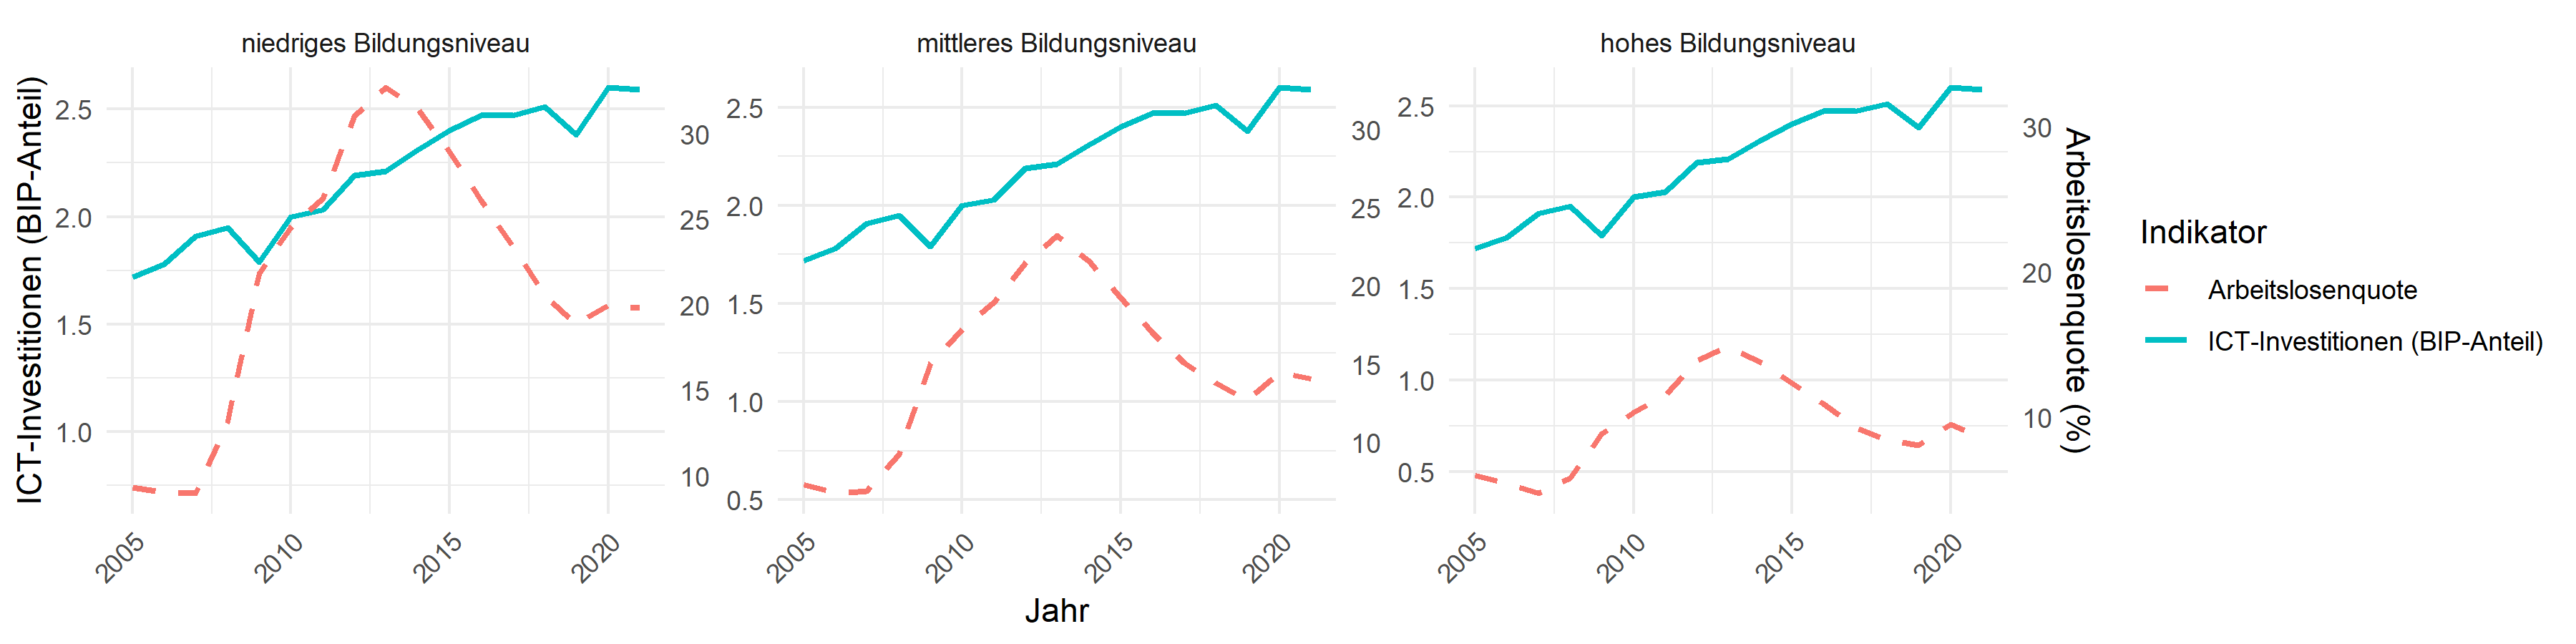
\includegraphics[width=\textwidth]{assets/plot_spain_final.png}
    \caption{Überblick über \textit{\ac{ICT}-Investitionen} und Arbeitslosenquote in 
    Spanien}
    \label{fig:spain}
\end{figure}

Die Abbildung zeigt die Entwicklung der \textit{\ac{ICT}-Investitionen} als Anteil am 
BIP sowie die Arbeitslosenquote in Spanien zwischen 2005 und 2022, differenziert nach 
Bildungsniveau - Spanien steht hier repräsentativ für südeuropäische Wohlfahrtsstaaten. 
Am Beispiel Spaniens ist ein besonders markanter Anstieg der Arbeitslosenquote während 
der Finanz- und Wirtschaftskrise von 2008 bis 2013 zu beobachten. Während die 
\textit{\ac{ICT}-Investitionen} einen insgesamt moderaten Anstieg über den gesamten 
Zeitraum hinweg zeigen, lassen sich drastische Schwankungen in der Arbeitslosenquote 
identifizieren, insbesondere bei Personen mit niedrigem und mittlerem Bildungsniveau.

Bei Personen mit einem niedrigen Bildungsniveau zeigt sich zwischen 2005 und 2008 
eine relativ stabile Arbeitslosenquote von knapp unter 10\%. Ab 2008 kam es jedoch zu 
einem rasanten Anstieg, der bis 2013 einen Höchststand von über 30\% erreichte. Erst 
nach 2013 begann ein kontinuierlicher Rückgang, der sich bis 2020 auf etwa 20\% 
fortsetzte, bevor ein erneuter leichter Anstieg zu beobachten ist. Die 
\textit{\ac{ICT}-Investitionen} entwickelten sich hingegen gleichmäßiger. Sie begannen 
auf einem niedrigen Niveau von etwa 1,75\% des BIP, zeigten nach der Finanzkriese ab 
2010 eine Aufwärtstendenz und stabilisierten sich nach 2015 bei etwa 2,5\%. Der 
Rückgang der Arbeitslosenquote nach 2013 verlief jedoch unabhängig von einer abrupten 
Zunahme der \textit{\ac{ICT}-Investitionen}, was darauf hindeutet, dass 
makroökonomische Faktoren (z. B. wirtschaftliche Erholung, Beschäftigungsprogramme) 
für die Senkung der Arbeitslosigkeit eine zentrale Rolle spielten.

Bei Personen mit mittlerem Bildungsniveau zeigt sich ein sehr ähnlicher Verlauf. Die 
Arbeitslosenquote lag 2005 noch unter 8\%, stieg im Zuge der Wirtschaftskrise bis 2013 
jedoch auf über 20\% an. Erst ab 2014 begann ein deutlicher Rückgang, der sich bis 
2020 auf etwa 10\% fortsetzte. Die \textit{\ac{ICT}-Investitionen} folgten hier einem 
vergleichbaren Muster wie in der Gruppe der gering Qualifizierten, wobei ein leichter, 
aber kontinuierlicher Anstieg sichtbar ist. Dennoch ist keine direkte Korrelation 
zwischen dem Verlauf der \textit{\ac{ICT}-Investitionen} und der Arbeitslosenquote 
ersichtlich, da der massive Anstieg und der spätere Rückgang der Arbeitslosigkeit 
primär durch die wirtschaftliche Entwicklung und nicht durch technologische 
Investitionen bedingt zu sein scheinen.

Bei Personen mit hohem Bildungsniveau war die Arbeitslosenquote insgesamt niedriger, 
zeigte jedoch ebenfalls einen deutlichen Anstieg während der Wirtschaftskrise. Im Jahr 
2005 lag sie unter 5\%, erreichte 2013 jedoch fast 15\%. Danach setzte auch hier ein 
Rückgang ein, und bis 2020 fiel die Quote auf etwa 5\% zurück. Im Gegensatz zu den 
anderen Bildungsgruppen scheinen sich hier die \textit{\ac{ICT}-Investitionen} und 
die Arbeitslosenquote teilweise gegenläufig zu entwickeln. Während die 
\textit{\ac{ICT}-Investitionen} nach 2010 eine stetige Steigerung zeigen und nach 
2015 stabil auf etwa 2,5\% des BIP bleiben, geht die Arbeitslosenquote in derselben 
Phase zurück. Dies könnte darauf hindeuten, dass hochqualifizierte Arbeitskräfte in 
Spanien stärker von der Digitalisierung profitieren konnten als Personen mit 
niedrigerem Bildungsstand.

Spanien als südeuropäischer Wohlfahrtsstaat ist durch einen stark segmentierten 
Arbeitsmarkt gekennzeichnet, der sich durch hohe Anteile an befristeten 
Beschäftigungsverhältnissen sowie eine geringere Arbeitsplatzsicherheit auszeichnet 
\parencite[vgl.][159–160]{bentolila2012two}. Dies könnte eine Erklärung für die starken 
Schwankungen der Arbeitslosenquote im Zuge der Finanzkrise sein, da insbesondere 
gering und mittel Qualifizierte von Entlassungen betroffen waren. Die 
\textit{\ac{ICT}-Investitionen} scheinen langfristig zwar leicht anzusteigen, doch zeigt 
sich kein direkter Zusammenhang zwischen diesen Investitionen und der Arbeitslosenquote 
in den jeweiligen Bildungsgruppen. Vielmehr deutet die Entwicklung darauf hin, dass der 
Arbeitsmarkt in Spanien stark konjunkturabhängig ist und die wirtschaftliche Erholung 
nach 2013 die wichtigste Triebkraft für die Reduktion der Arbeitslosigkeit war 
\parencite[vgl.][157–159]{bentolila2012two}.

Zusammenfassend zeigen die Daten für Spanien eine enge Verbindung zwischen der 
Finanzkrise und den massiven Schwankungen der Arbeitslosenquote, insbesondere bei 
gering und mittel Qualifizierten. Während \textit{\ac{ICT}-Investitionen} über den 
Zeitraum hinweg einen kontinuierlichen, aber moderaten Anstieg zeigen, sind ihre 
direkten Auswirkungen auf die Arbeitslosigkeit unklar. Es könnte jedoch sein, dass 
insbesondere Hochqualifizierte von den steigenden \textit{\ac{ICT}-Investitionen} 
profitieren konnten, während gering Qualifizierte eher von konjunkturellen 
Faktoren abhängig waren.

% Deskriptive Analyse: Grafik "Polen"
\begin{figure}[htbp]
    \centering
    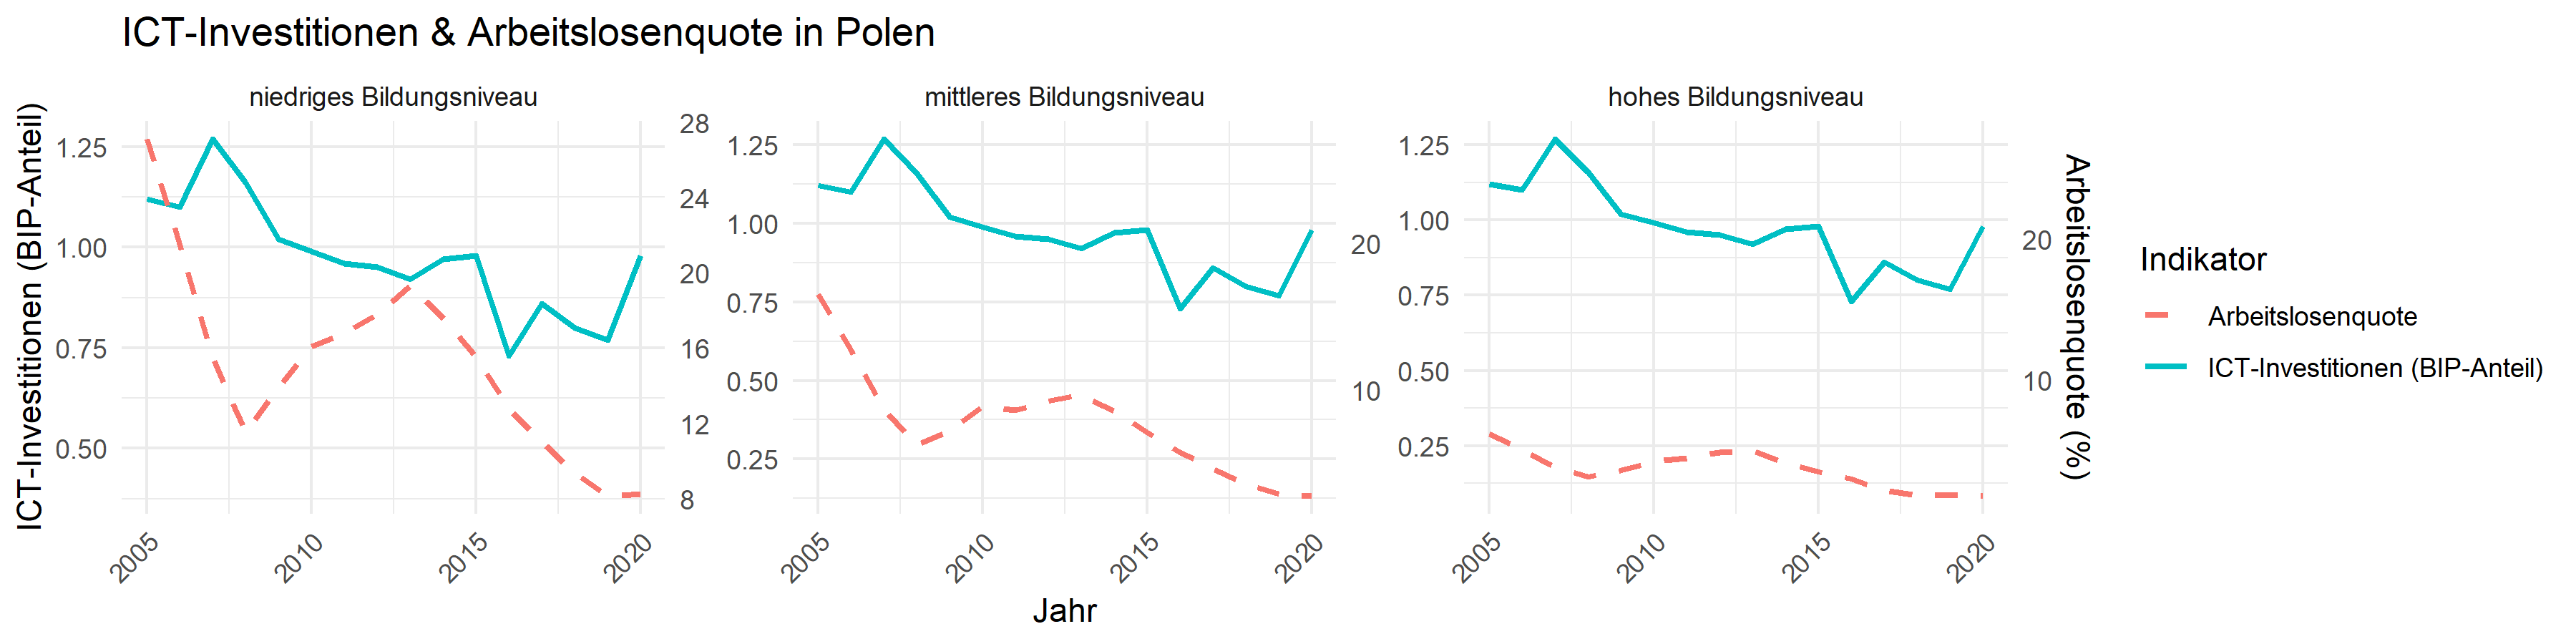
\includegraphics[width=\textwidth]{assets/plot_poland_final.png}
    \caption{Überblick über \textit{\ac{ICT}-Investitionen} und Arbeitslosenquote 
    in Polen}
    \label{fig:poland}
\end{figure}

Die Abbildung zeigt die Entwicklung der \textit{\ac{ICT}-Investitionen} als Anteil 
am BIP sowie die Arbeitslosenquote in Polen zwischen 2005 und 2022 differenziert 
nach Bildungsniveau - Polen steht hier repräsentativ für postsozialistische 
Wohlfahrtsstaaten.

Auffällig ist der durchgängige Rückgang der Arbeitslosenquote in allen 
Bildungsgruppen, während die \textit{\ac{ICT}-Investitionen} über weite Strecken 
konstant bleiben, beziehungsweise sogar ebenfalls einen Rückgang verzeichnen. Dies 
deutet darauf hin, dass makroökonomische oder arbeitsmarktpolitische Faktoren für 
den Rückgang der Arbeitslosigkeit maßgeblich verantwortlich sein könnten.

Bei Personen mit einem niedrigen Bildungsniveau lag die Arbeitslosenquote im Jahr 
2005 bei knapp 28\%. In den darauffolgenden Jahren kam es zu einem raschen Rückgang, 
wobei jedoch zwischen 2010 und 2015 eine Stagnation mit einem kurzen Anstieg auf fast 
20\% zu beobachten ist. Nach 2015 setzte sich der Rückgang der Arbeitslosenquote 
fort, sodass sie bis 2020 auf 8\% fiel. Die \textit{\ac{ICT}-Investitionen} blieben 
über den gesamten Zeitraum hinweg weitgehend konstant und bewegten sich um die 1\% des 
BIP, mit einem leichten Rückgang zwischen 2010 und 2015. Dies deutet darauf hin, dass  
der starke Rückgang der Arbeitslosigkeit nicht direkt mit den 
\textit{\ac{ICT}-Investitionen} zusammenhängt, sondern durch andere wirtschaftliche 
Faktoren beeinflusst wurde, beispielsweise durch eine allgemeine wirtschaftliche 
Stabilisierung nach dem EU-Beitritt Polens und steigende Beschäftigungsmöglichkeiten 
in arbeitsintensiven Branchen.

Für Personen mit einem mittleren Bildungsniveau zeigt sich ein ähnliches Muster, wenn 
auch auf einem insgesamt niedrigeren Ausgangsniveau der Arbeitslosenquote. Während 
diese 2005 noch über 10\% lag, sank sie in den darauffolgenden Jahren rasch auf etwa 
3\% bis 2015 und weiter unter 2\% bis 2020. Zwischen 2010 und 2015 ist jedoch eine 
leichte Erhöhung der Arbeitslosenquote erkennbar, bevor der Trend weiter nach unten 
verlief. Der Rückgang der Arbeitslosigkeit erfolgt weitgehend unabhängig von der 
Entwicklung der \textit{\ac{ICT}-Investitionen}, was darauf hindeutet, dass 
makroökonomische Faktoren wie die Industrialisierung und eine steigende Nachfrage 
nach Arbeitskräften mit mittlerer Qualifikation eine bedeutendere Rolle gespielt 
haben könnten.

Für Personen mit einem hohen Bildungsniveau war die Arbeitslosenquote bereits 
2005 relativ niedrig, lag aber dennoch bei etwa 6\%, was im Vergleich zu anderen 
europäischen Ländern eher hoch ist. Dies könnte auf strukturelle Faktoren des 
polnischen Arbeitsmarktes zurückzuführen sein, wie eine geringere Anzahl 
hochqualifizierter Beschäftigungsmöglichkeiten in den frühen 2000er-Jahren. In den 
darauffolgenden Jahren fiel die Arbeitslosenquote jedoch deutlich und lag bereits 
2015 unter 2\%. Auffällig ist, dass die \textit{\ac{ICT}-Investitionen} in dieser 
Gruppe im Gegensatz zu den anderen Bildungsgruppen eine leichte Steigerung zeigen. 
In der ersten Hälfte des Beobachtungszeitraums bewegten sich die 
\textit{\ac{ICT}-Investitionen} um 1,2\% des BIP, während sie in den Jahren nach 
2015 tendenziell anstiegen. Dies könnte darauf hindeuten, dass der polnische 
Arbeitsmarkt mit steigendem ICT-Investitionsanteil zunehmend hochqualifizierte 
Beschäftigungsmöglichkeiten geschaffen hat. Dennoch bleibt die Kausalität unklar, 
da die Arbeitslosenquote in dieser Gruppe bereits gefallen war, bevor der leichte 
Anstieg der \textit{\ac{ICT}-Investitionen} einsetzte.

Polen als postsozialistischer Wohlfahrtsstaat hat in den letzten Jahrzehnten einen 
tiefgreifenden wirtschaftlichen Wandel durchlaufen. Der EU-Beitritt im Jahr 2004 
führte zu verstärkten ausländischen Direktinvestitionen, einer zunehmenden 
Integration in europäische Produktionsnetzwerke sowie einer generellen 
Modernisierung der Wirtschaft. Diese Entwicklungen spiegeln sich auch in der 
Reduktion der Arbeitslosigkeit wider, die in allen Bildungsgruppen signifikant 
gesunken ist. Besonders bei Personen mit mittlerem und niedrigem Bildungsniveau 
könnte die Expansion von Industriejobs sowie der Dienstleistungssektor eine 
wesentliche Rolle gespielt haben \parencite[vgl.][S. 455–459]{myant2013transition}.

Insgesamt zeigt die Abbildung, dass die Arbeitslosenquote in allen Bildungsgruppen 
stark gesunken ist, während die \textit{\ac{ICT}-Investitionen} nur moderate 
Schwankungen aufweisen. Dies deutet darauf hin, dass die Haupttreiber der 
Beschäftigungsentwicklung in Polen eher in wirtschaftlichen und 
arbeitsmarktpolitischen Veränderungen zu suchen sind als in den direkten 
Auswirkungen von \textit{\ac{ICT}-Investitionen}. Dennoch könnte die leichte 
Zunahme der \textit{\ac{ICT}-Investitionen} im späteren Beobachtungszeitraum 
darauf hinweisen, dass sich der polnische Arbeitsmarkt allmählich in Richtung 
einer wissensbasierten Wirtschaft entwickelt, in der besonders Hochqualifizierte 
profitieren.

% Deskriptive Analyse: Grafik "Schweden"
\begin{figure}[htbp]
    \centering
    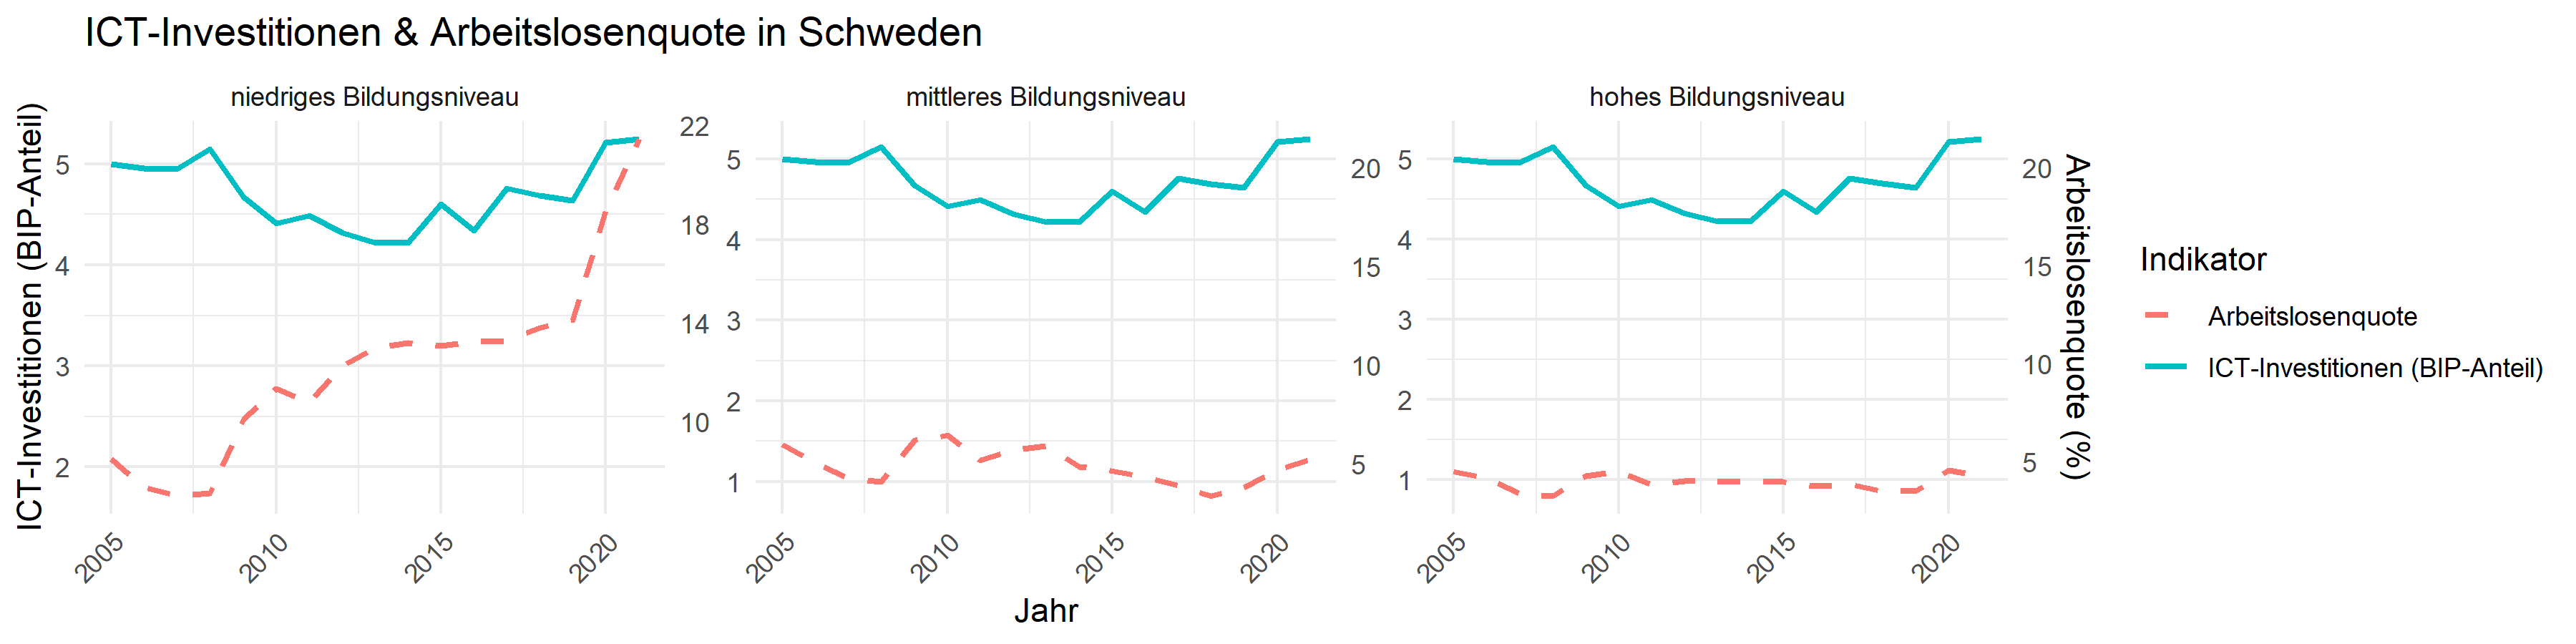
\includegraphics[width=\textwidth]{assets/plot_sweden_final.png}
    \caption{Überblick über \textit{\ac{ICT}-Investitionen} und Arbeitslosenquote in 
    Schweden}
    \label{fig:sweden}
\end{figure}

Die Abbildung zeigt die Entwicklung der \textit{\ac{ICT}-Investitionen} als Anteil 
am BIP sowie die Arbeitslosenquote in Schweden zwischen 2005 und 2022, differenziert 
nach Bildungsniveau - Schweden steht hier repräsentativ für nordische 
Wohlfahrtsstaaten. Im Gegensatz zu anderen Ländern ist hier eine relativ stabile 
Entwicklung der Arbeitslosenquote über den gesamten Zeitraum zu beobachten, mit nur 
moderaten Schwankungen. Auffällig ist zudem, dass die \textit{\ac{ICT}-Investitionen} 
in Schweden im internationalen Vergleich auf einem vergleichsweise hohen Niveau liegen. 
Während sie in der ersten Dekade leichte Schwankungen zeigen, bleibt ihr Niveau ab 
2010 weitgehend konstant und steigt gegen Ende des Betrachtungszeitraums leicht an.

Bei Personen mit einem niedrigen Bildungsniveau lag die Arbeitslosenquote 2005 bei knapp 
5\% und zeigte bis etwa 2010 einen moderaten Anstieg. Nach 2010 stabilisierte sich die 
Arbeitslosenquote zunächst, bevor sie ab 2015 einen erneuten Aufwärtstrend verzeichnete. 
Besonders auffällig ist der deutliche Anstieg nach 2018, der sich bis 2022 fortsetzt. 
Während die Arbeitslosenquote für gering Qualifizierte also in den letzten Jahren 
gestiegen ist, sind die \textit{\ac{ICT}-Investitionen} im selben Zeitraum weitgehend 
stabil geblieben, wenn auch mit einer leicht positiven Tendenz. Dies könnte darauf 
hindeuten, dass die fortschreitende Digitalisierung möglicherweise die 
Beschäftigungsmöglichkeiten für niedrig qualifizierte Arbeitskräfte verschlechtert hat, 
indem sie bestimmte Arbeitsplätze verdrängte oder die Anforderungen an digitale 
Kompetenzen erhöhte - wahrscheinlich hängt diese Beobachtung aber eher mit der 
Corona-Pandemie zusammen.

Für Personen mit einem mittleren Bildungsniveau zeigt sich ein stabiles Muster, mit 
einer weitgehend konstanten Arbeitslosenquote zwischen 2005 und 2018. Während die 
Arbeitslosigkeit 2005 bei unter 5\% lag, gab es bis 2015 eine leichte Abwärtsbewegung, 
gefolgt von einer weitgehenden Stabilisierung. Nach 2018 zeigt sich eine leicht steigende 
Tendenz der Arbeitslosenquote, wenn auch weniger ausgeprägt als bei den gering 
Qualifizierten. Die \textit{\ac{ICT}-Investitionen} sind in dieser Gruppe durchgängig 
hoch und zeigen eine stabile Entwicklung mit leichten Schwankungen. Anders als bei den 
gering Qualifizierten ist hier keine klare gegenläufige Entwicklung zwischen 
\textit{\ac{ICT}-Investitionen} und Arbeitslosigkeit zu erkennen, was darauf hindeutet, 
dass mittlere Qualifikationen in Schweden weniger stark von den technologischen 
Veränderungen betroffen sind.

Bei Personen mit einem hohen Bildungsniveau zeigt sich über den gesamten Zeitraum 
hinweg eine extrem niedrige Arbeitslosenquote. Bereits 2005 lag sie unter 5\% und blieb 
über den gesamten Zeitraum stabil, mit nur minimalen Schwankungen. Auffällig ist, dass 
die \textit{\ac{ICT}-Investitionen} in dieser Gruppe im internationalen Vergleich sehr 
hoch sind, mit Werten, die konstant bei 4-5\% des \ac{BIP} liegen. Die Kombination aus 
hoher \ac{ICT}-Investition und niedriger Arbeitslosenquote deutet darauf hin, dass 
hochqualifizierte Arbeitskräfte in Schweden stark von der Digitalisierung profitieren 
konnten. Dies entspricht auch theoretischen Erwartungen, da hochqualifizierte 
Beschäftigte in wissensintensiven Branchen tätig sind, die von technologischen 
Innovationen profitieren.

Die stabilen \textit{\ac{ICT}-Investitionen} und die insgesamt niedrigen Arbeitslosenquoten 
deuten darauf hin, dass der schwedische Arbeitsmarkt relativ widerstandsfähig gegenüber 
technologischen Veränderungen ist. Allerdings lässt sich bei niedrig qualifizierten 
Arbeitskräften ein Anstieg der Arbeitslosigkeit nach 2018 beobachten, der 
möglicherweise mit strukturellen Veränderungen auf dem Arbeitsmarkt zusammenhängt. 
Dies könnte darauf hindeuten, dass bestimmte Berufe durch die Digitalisierung 
zunehmend verdrängt werden oder dass sich die Anforderungen an digitale Kompetenzen 
verstärkt haben, sodass Geringqualifizierte Schwierigkeiten haben, sich an die 
veränderten Bedingungen anzupassen.

Insgesamt zeigt die Abbildung, dass Schweden ein stabiles Beschäftigungsniveau über 
den gesamten Zeitraum hinweg aufweist, wobei die \textit{\ac{ICT}-Investitionen} 
konstant hoch sind. Während Hoch- und Mittelqualifizierte weitgehend von den 
Entwicklungen profitieren konnten, scheint sich für gering Qualifizierte in den 
letzten Jahren eine Verschlechterung der Beschäftigungssituation abzuzeichnen. Dies 
könnte darauf hindeuten, dass Digitalisierung in hochentwickelten Volkswirtschaften 
wie Schweden zunehmend zu einer Polarisierung des Arbeitsmarktes führt, bei der 
Hochqualifizierte von den Investitionen profitieren, während gering Qualifizierte 
zunehmend unter Druck geraten.

% Deskriptive Analyse: Grafik "Deutschland"
\begin{figure}[htbp]
    \centering
    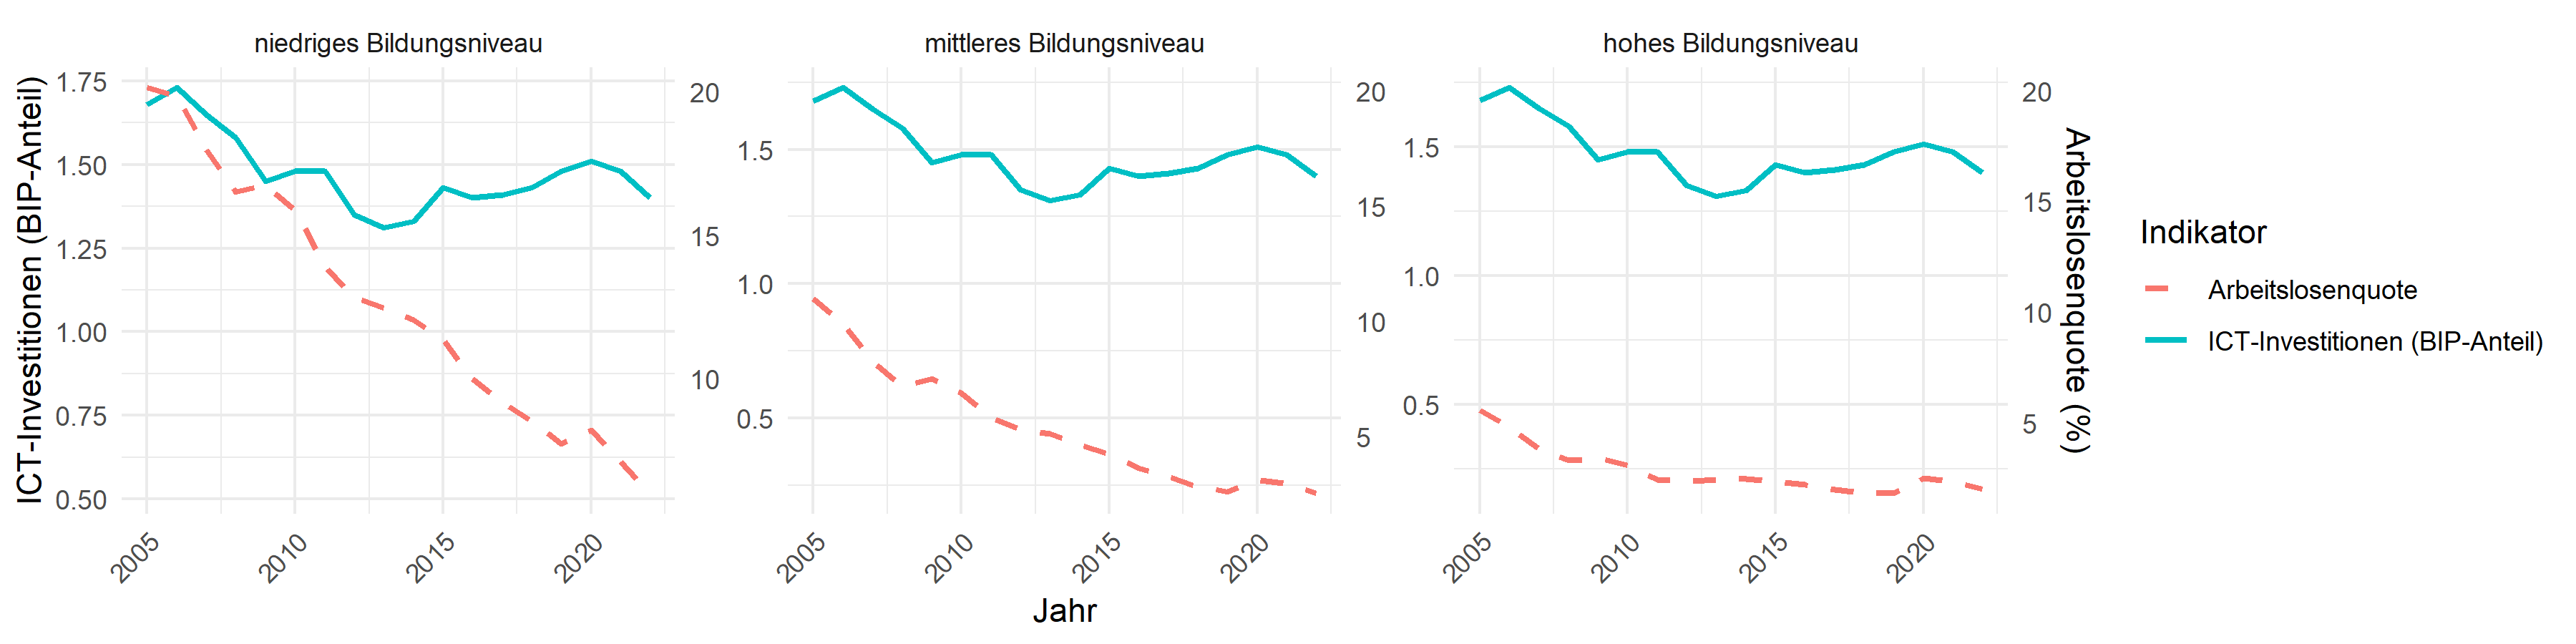
\includegraphics[width=\textwidth]{assets/plot_germany_final.png}
    \caption{Überblick über \textit{\ac{ICT}-Investitionen} und Arbeitslosenquote in 
    Deutschland}
    \label{fig:germany}
\end{figure}

Die Abbildung zeigt die Entwicklung der \textit{\ac{ICT}-Investitionen} als Anteil 
am BIP sowie die Arbeitslosenquote in Deutschland zwischen 2005 und 2022, 
differenziert nach Bildungsniveau - Deutschland steht hier repräsentativ für 
mitteleuropäische Wohlfahrtsstaaten. Dabei lassen sich klare Unterschiede zwischen 
den drei betrachteten Gruppen - niedriges, mittleres und hohes Bildungsniveau - sowohl 
hinsichtlich des Niveaus als auch der Veränderung der Arbeitslosenquoten erkennen. 
Insgesamt zeigen sich über den gesamten Zeitraum hinweg deutliche Rückgänge in der 
Arbeitslosenquote, während die \textit{\ac{ICT}-Investitionen} eine weitgehend 
stabile Entwicklung aufweisen.

Für Personen mit einem niedrigen Bildungsniveau zeigt sich eine besonders hohe 
Arbeitslosenquote zu Beginn des Beobachtungszeitraums, die 2005 bei über 18\% lag. 
In den darauffolgenden Jahren kam es zu einem kontinuierlichen Rückgang, der bis 2020 
Werte unter 5\% erreichte. Diese Entwicklung spiegelt die allgemeine Verbesserung des 
deutschen Arbeitsmarktes wider, insbesondere durch wirtschaftlichen Aufschwung und 
Reformen im Rahmen der Agenda 2010. Die \textit{\ac{ICT}-Investitionen} verzeichneten 
zwischen 2005 und 2010 zunächst einen leichten Rückgang, bevor sie sich um die 1,5\% 
des BIP stabilisierten. Ein direkter Zusammenhang zwischen 
\textit{\ac{ICT}-Investitionen} und der sinkenden Arbeitslosenquote ist nicht 
ersichtlich, da der Rückgang der Arbeitslosenquote bereits vor der leichten 
Stabilisierung der Investitionen begann.

Bei Personen mit mittlerem Bildungsniveau zeigt sich ein ähnliches Muster, wenn auch 
auf einem insgesamt niedrigeren Ausgangsniveau der Arbeitslosenquote. Während diese 
2005 noch bei etwa 10\% lag, fiel sie bis 2020 auf rund 3\% und blieb seither 
weitgehend stabil. Die \textit{\ac{ICT}-Investitionen} zeigen eine konstante 
Entwicklung mit geringen Schwankungen. Auch hier bleibt der direkte Zusammenhang 
zwischen den \textit{\ac{ICT}-Investitionen} und der Arbeitslosenquote unklar, da 
der Rückgang der Arbeitslosigkeit langfristig verläuft und nicht direkt mit den 
Investitionen korreliert.

Für Personen mit hohem Bildungsniveau zeigt sich über den gesamten Zeitraum hinweg 
eine sehr niedrige Arbeitslosenquote. Bereits 2005 lag sie unter 5\% und sank bis
2010 auf unter 2\%, wo sie anschließend auf diesem niedrigen Niveau stabil blieb. 
Im Vergleich zu den anderen Bildungsgruppen weist diese Gruppe somit die geringsten 
Schwankungen auf. Die \textit{\ac{ICT}-Investitionen} zeigen auch hier eine 
weitgehend stabile Entwicklung. Dies könnte darauf hindeuten, dass Hochqualifizierte 
vermehrt in Berufen tätig sind, die von steigenden \textit{\ac{ICT}-Investitionen} 
profitieren, jedoch bleibt auch hier die Kausalität unklar.

Deutschland als konservativer Wohlfahrtsstaat zeichnet sich durch eine enge Verzahnung 
von Bildungssystem und Arbeitsmarkt aus \parencite[vgl.][S. 21–22]{hall2001varieties}. 
Insbesondere das duale Ausbildungssystem und gezielte arbeitsmarktpolitische Maßnahmen 
könnten eine Rolle beim Rückgang der 
Arbeitslosenquoten in den niedrigen und mittleren Bildungsgruppen gespielt haben. 
Die \textit{\ac{ICT}-Investitionen} zeigen über den Beobachtungszeitraum hinweg keine 
drastischen Veränderungen, was darauf hindeutet, dass technologische Entwicklungen 
schrittweise in den Arbeitsmarkt integriert wurden. Besonders für Hochqualifizierte 
könnte eine steigende Nachfrage nach digitalen Fähigkeiten eine Rolle gespielt 
haben, während bei den niedrigen und mittleren Bildungsniveaus der 
Arbeitsmarktrückgang vermutlich durch andere makroökonomische Faktoren beeinflusst 
wurde.

Die Abbildung verdeutlicht insgesamt, dass die Arbeitslosenquoten in allen 
Bildungsgruppen über die Jahre hinweg gesunken sind, während die 
\textit{\ac{ICT}-Investitionen} vergleichsweise stabil geblieben sind. Dies lässt darauf 
schließen, dass der Rückgang der Arbeitslosigkeit nicht direkt durch 
\textit{\ac{ICT}-Investitionen} getrieben wurde, sondern eher mit makroökonomischen 
Entwicklungen und strukturellen Veränderungen auf dem deutschen Arbeitsmarkt 
zusammenhängt.

% Deskriptive Analyse: Grafik "Großbritannien"
\begin{figure}[htbp]
    \centering
    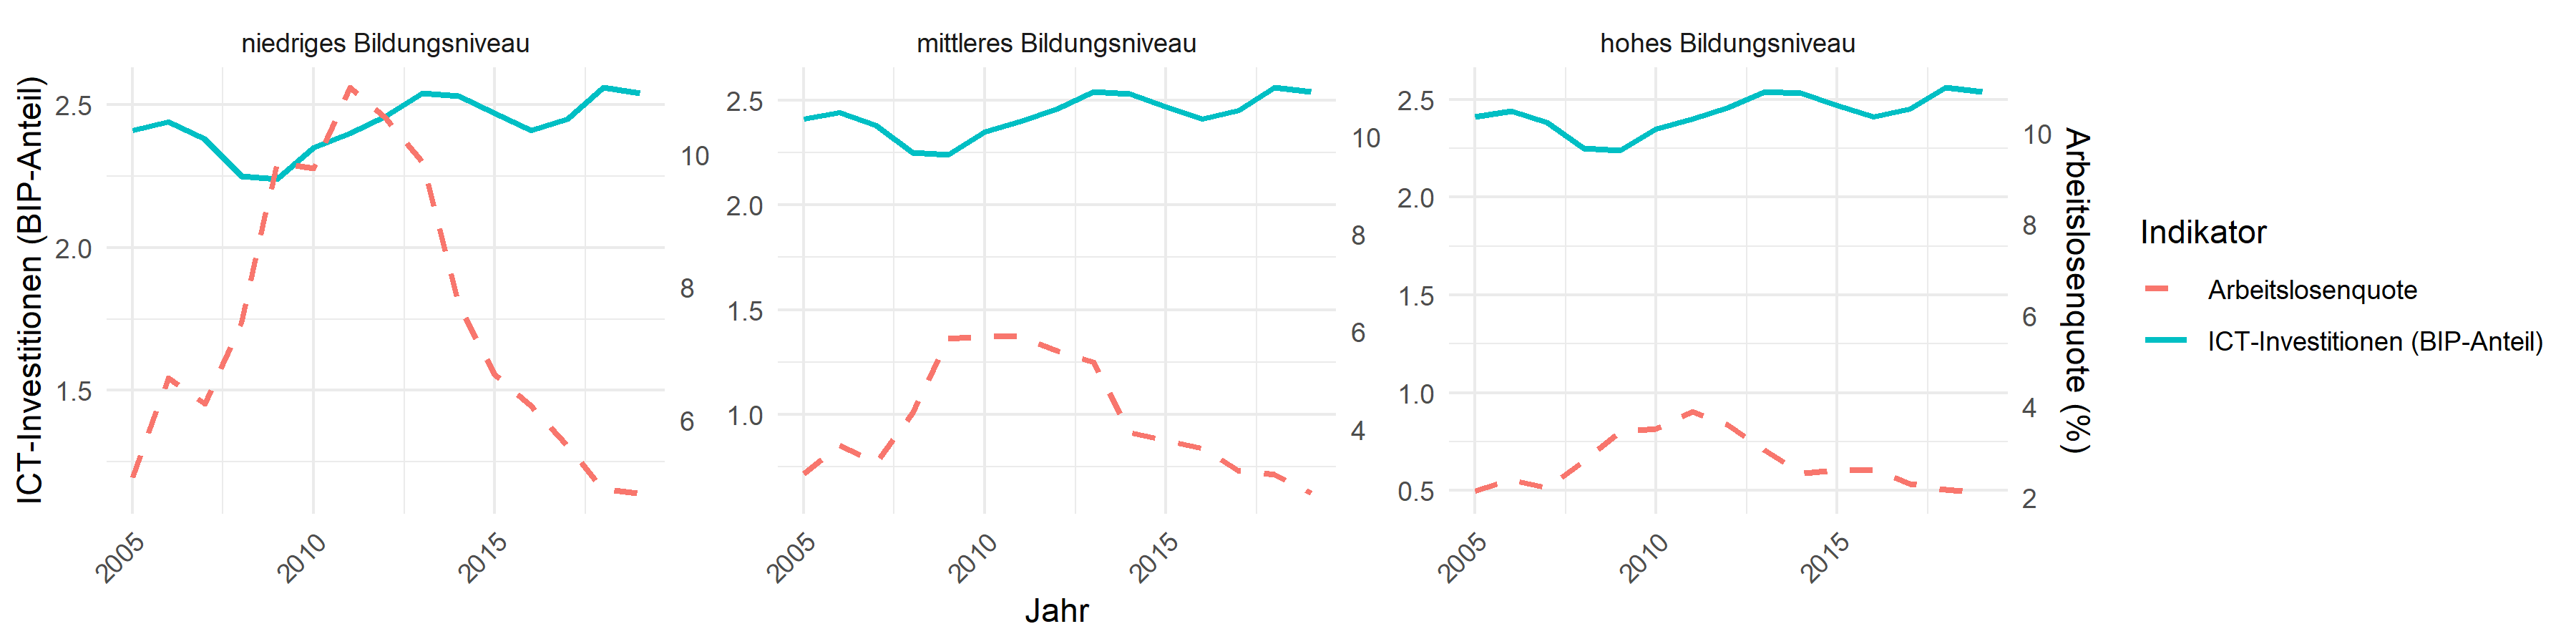
\includegraphics[width=\textwidth]{assets/plot_uk_final.png}
    \caption{Überblick über \textit{\ac{ICT}-Investitionen} und Arbeitslosenquote in 
    Großbritannien}
    \label{fig:uk}
\end{figure}

Die Abbildung zeigt die Entwicklung der \textit{\ac{ICT}-Investitionen} als Anteil am BIP 
sowie die Arbeitslosenquote in Großbritannien zwischen 2005 und 2022, differenziert nach 
Bildungsniveau - Großbritannien steht hier repräsentativ für angelsächsische 
Wohlfahrtsstaaten. Im Vergleich zu anderen Wohlfahrtsstaatentypen weist Großbritannien eine 
relativ konstante Arbeitslosenquote auf, die über den Zeitraum hinweg nur leichte 
Rückgänge zeigt. Auffällig ist, dass die \textit{\ac{ICT}-Investitionen} in Großbritannien 
zwar einen moderaten Anstieg aufweisen, sich jedoch auf einem relativ niedrigen Niveau 
bewegen.

Bei Personen mit einem niedrigen Bildungsniveau lag die Arbeitslosenquote im Jahr 2005 
bei etwa 8\% und sank bis 2020 auf unter 4\%. Anders als in Ländern mit stärker 
regulierten Arbeitsmärkten zeigt sich hier kein abrupter Rückgang, sondern eine 
schrittweise Anpassung über den Zeitraum hinweg. Gleichzeitig zeigen die 
\textit{\ac{ICT}-Investitionen} einen leicht steigenden Trend, bleiben jedoch im Bereich 
von etwa 1,5\% des BIP. Ein klarer Zusammenhang zwischen \textit{\ac{ICT}-Investitionen} 
und der Arbeitslosenquote lässt sich nicht unmittelbar erkennen, was darauf hindeuten 
könnte, dass andere arbeitsmarktpolitische oder wirtschaftliche Faktoren maßgeblicher für 
die Reduktion der Arbeitslosigkeit sind.

Bei Personen mit mittlerem Bildungsniveau zeigt sich ein ähnliches Muster. Die 
Arbeitslosenquote lag 2005 bei etwa 6\% und fiel bis 2015 auf rund 3\%, wo sie sich 
anschließend stabilisierte. Die \textit{\ac{ICT}-Investitionen} zeigen hier eine geringe 
Zunahme, bleiben jedoch weitgehend konstant im Bereich von 1,5\% bis 2\% des BIP. Auch in 
dieser Gruppe scheint der Rückgang der Arbeitslosenquote eher mit marktwirtschaftlichen 
Anpassungen als mit direkten Effekten der \textit{\ac{ICT}-Investitionen} zusammenzuhängen. 
Der relativ geringe Anstieg der Investitionen deutet darauf hin, dass die britische 
Wirtschaft zwar technologische Entwicklungen integriert, jedoch nicht in dem Ausmaß wie 
andere hochdigitalisierte Volkswirtschaften.

Für Personen mit hohem Bildungsniveau zeigt sich über den gesamten Zeitraum hinweg eine 
sehr niedrige Arbeitslosenquote. Bereits 2005 lag sie unter 3\% und blieb über den 
gesamten Zeitraum weitgehend stabil, mit nur minimalen Schwankungen. Die 
\textit{\ac{ICT}-Investitionen} zeigen auch hier eine relativ konstante Entwicklung, 
liegen jedoch ebenfalls im Bereich von 1,5\% bis 2\% des BIP. Dies deutet darauf hin, 
dass Hochqualifizierte kaum von negativen Beschäftigungseffekten durch Digitalisierung 
betroffen sind. Vielmehr könnte der flexible britische Arbeitsmarkt es dieser Gruppe 
erleichtert haben, sich an technologische Veränderungen anzupassen.

Großbritannien als anglo-sächsischer Wohlfahrtsstaat zeichnet sich durch einen 
weniger regulierten Arbeitsmarkt aus, der sich durch eine hohe Flexibilität und eine 
geringere staatliche Intervention auszeichnet \parencite[vgl.][S. 21]{trabert1997entwicklung}. 
Diese Charakteristik könnte erklären, warum die Arbeitslosenquoten über den Zeitraum hinweg 
relativ stabil bleiben und gleichzeitig keine drastischen Veränderungen im Bereich der 
\textit{\ac{ICT}-Investitionen} feststellbar sind. Der moderate Rückgang der Arbeitslosigkeit 
deutet darauf hin, dass sich der britische Arbeitsmarkt schrittweise an Digitalisierung angepasst 
hat, ohne dass bestimmte Gruppen massiv benachteiligt wurden.

Zusammenfassend zeigt die Abbildung, dass sich die britische Arbeitslosenquote über die 
Jahre hinweg in allen Bildungsgruppen verringert hat, wenn auch nicht so drastisch wie in 
anderen Ländern. Gleichzeitig bleiben die \textit{\ac{ICT}-Investitionen} auf einem 
relativ niedrigen Niveau und zeigen keine unmittelbare Korrelation mit den Veränderungen 
der Arbeitslosenquote. Dies deutet darauf hin, dass makroökonomische Faktoren wie die 
Arbeitsmarktflexibilität und allgemeine wirtschaftliche Entwicklung eine wichtigere Rolle 
für die Beschäftigungsdynamik spielen als allein die Höhe der \textit{\ac{ICT}-Investitionen}.


%%%%%%%%%%%%%%%%%%%%%%%%%
% Multivariate Analysen %
%%%%%%%%%%%%%%%%%%%%%%%%%

\subsection{Multivariate Analysen}

% Multivariate Analyse: Einleitung
Die Zusammenfassung der Ergebnisse aus den Modellen mit Kontrollvariablen zeigt eine 
umfassende, jedoch differenzierte Analyse der Auswirkungen von 
\textit{\ac{ICT}-Investitionen} auf die Arbeitslosenquote in den drei Bildungsgruppen 
(„niedriges Bildungsniveau“, „mittleres Bildungsniveau“, „hohes Bildungsniveau“). Die
Modelle liefern wichtige Hinweise auf die Bedeutung makroökonomischer Rahmenbedingungen
und institutioneller Strukturen, während der direkte Einfluss von
\textit{\ac{ICT}-Investitionen} signifikant, aber unterschiedlich stark ausfällt.

% Multivariate Analyse: Modelle ohne Interaktion
% TODO: - (Stand 04.03.2025)

\begin{table}[H]
\caption{Einzelwerte der Regressionsmodellparameter für die Kontrollmodelle}
\resizebox{\textwidth}{!}{
\centering
\begin{talltblr}[         %% tabularray outer open
entry=none,label=none,
note{}={+ p \num{< 0.1}, * p \num{< 0.05}, ** p \num{< 0.01}, *** p \num{< 0.001}},
]                     %% tabularray outer close
{                     %% tabularray inner open
colspec={Q[]Q[]Q[]Q[]},
column{2,3,4}={}{halign=c,},
column{1}={}{halign=l,},
hline{13}={1,2,3,4}{solid, black, 0.05em},
}                     %% tabularray inner close
\toprule
& niedriges
Bildungsniv.
(Kontrolle) & mittleres
Bildungsniv.
(Kontrolle) & hohes
Bildungsniv.
(Kontrolle) \\ \midrule %% TinyTableHeader
ICT\_INVEST\_SHARE\_GDP     & \num{2.302}***  & \num{1.157}***  & \num{0.455}***  \\
& (\num{0.232})   & (\num{0.146})   & (\num{0.086})   \\
GDP\_PER\_CAPITA             & \num{-0.194}*** & \num{-0.153}*** & \num{-0.083}*** \\
& (\num{0.018})   & (\num{0.012})   & (\num{0.007})   \\
PERCENT\_TERTIARY\_EDUCATION & \num{0.606}***  & \num{0.282}***  & \num{0.140}***  \\
& (\num{0.052})   & (\num{0.032})   & (\num{0.019})   \\
REGULATION\_STRICTNESS        & \num{-0.147}    & \num{-0.118}*   & \num{-0.085}*   \\
& (\num{0.094})   & (\num{0.059})   & (\num{0.035})   \\
PERCENT\_EMPLOYEES\_TUD      & \num{0.128}**   & \num{0.106}***  & \num{0.025}+    \\
& (\num{0.039})   & (\num{0.025})   & (\num{0.015})   \\
YEAR\_FACTOR & True & True & True \\
Num.Obs.                       & \num{3973}      & \num{3973}      & \num{3973}      \\
R2                             & \num{0.304}     & \num{0.308}     & \num{0.281}     \\
R2 Adj.                        & \num{0.295}     & \num{0.299}     & \num{0.272}     \\
AIC                            & \num{21393.1}   & \num{17747.2}   & \num{13530.6}   \\
BIC                            & \num{21537.7}   & \num{17891.8}   & \num{13675.2}   \\
RMSE                           & \num{3.55}      & \num{2.25}      & \num{1.32}      \\
\bottomrule
\end{talltblr}
}
\label{tab:models_control}
\end{table}


% Multivariate Analyse: Modell ohne Interaktion (niedriges Bildungsniveau)
Im Modell für die Gruppe mit niedrigem Bildungsniveau zeigt der geschätzte Koeffizient
für \textit{\ac{ICT}-Investitionen} einen positiven Wert von 2,302*** (p < 0,001), was auf
einen signifikanten positiven Zusammenhang zwischen \ac{ICT}-Investitionen und der
Arbeitslosenquote dieser Gruppe hindeutet. Dies bedeutet, dass in Ländern mit
höheren \ac{ICT}-Investitionen die Arbeitslosigkeit unter geringqualifizierten Personen
tendenziell ansteigt. Dies bestätigt die Hypothese, dass gering Qualifizierte stärker von
den negativen Effekten der Digitalisierung betroffen sind.

Das \textit{\ac{BIP} pro Kopf} zeigt mit einem Koeffizienten von -0,194*** (p < 0,001)
einen stark negativen und signifikanten Einfluss. Dies weist darauf hin, dass in wohlhabenderen
Ländern die Arbeitslosenquote für geringqualifizierte Personen tendenziell niedriger ist,
möglicherweise aufgrund eines breiteren Angebots an Beschäftigungsmöglichkeiten oder
arbeitsmarktpolitischer Maßnahmen.

Der \textit{Tertiärer Bildungsanteil} hat einen signifikanten positiven Effekt von 0,606**
(p < 0,01), was darauf hindeutet, dass eine höhere Bildungsbeteiligung in der Gesamtbevölkerung
zu strukturellen Veränderungen des Arbeitsmarktes führt, die auch auf geringqualifizierte Arbeitskräfte
Auswirkungen haben könnten. Die \textit{Gewerkschaftsdichte} weist mit einem Koeffizienten von 0,128**
(p < 0,01) einen signifikanten positiven Zusammenhang auf, was darauf hindeutet, dass eine höhere
gewerkschaftliche Organisationsrate mit einer leicht höheren Arbeitslosenquote für diese Gruppe
einhergeht. Die \textit{Regulierungsstrenge des Arbeitsmarkts} zeigt keinen signifikanten Effekt für
diese Gruppe.

% Multivariate Analyse: Modell ohne Interaktion (mittleres Bildungsniveau)
Für das mittlere Bildungsniveau ergibt sich ebenfalls ein signifikanter positiver Zusammenhang
zwischen \textit{\ac{ICT}-Investitionen} und Arbeitslosigkeit. Der geschätzte Koeffizient beträgt
1,157*** (p < 0,001), was darauf hindeutet, dass höhere \ac{ICT}-Investitionen mit einer steigenden
Arbeitslosigkeit in dieser Gruppe verbunden sind. Dies bestätigt die Hypothese, dass mittelqualifizierte
Arbeitskräfte ebenfalls von negativen Effekten der Digitalisierung betroffen sein können, wenn auch in
gerigerem Maße als geringqualifizierte Personen.

Das \textit{\ac{BIP} pro Kopf} zeigt mit einem Koeffizienten von -0,153*** (p < 0,001) einen signifikanten
negativen Zusammenhang. Dies deutet darauf hin, dass eine höhere Wirtschaftsleistung mit einer geringeren
Arbeitslosenquote für mittelqualifizierte Personen verbunden ist, vermutlich aufgrund eines stabileren
Arbeitsmarktes und größerer Weiterbildungsmöglichkeiten.

Der \textit{Tertiärer Bildungsanteil} weist einen signifikanten positiven Effekt von 0,282**
(p < 0,01) auf, was darauf hindeutet, dass eine höhere tertiäre Bildungsbeteiligung mit strukturellen
Arbeitsmarktveränderungen einhergeht, die möglicherweise den Druck auf mittelqualifizierte Berufe erhöhen.
Die \textit{Gewerkschaftsdichte} zeigt mit einem Koeffizienten von 0,106*** (p < 0,001) eine signifikante
positive Korrelation mit der Arbeitslosenquote, was darauf hindeutet, dass eine stärkere gewerkschaftliche
Organisationsrate nicht zwangsläufig zu niedrigeren Arbeitslosenquoten in dieser Gruppe führt. Die
\textit{Regulierungsstrenge des Arbeitsmarkts} hat einen signifikant negativen Effekt von -0,118*
(p < 0,05), was darauf hindeutet, dass strengere Arbeitsmarktregulierungen für diese Gruppe
stabilisierend wirken könnten, indem sie den Arbeitsplatzverlust für mittelqualifizierte Beschäftigte 
reduzieren.

% Multivariate Analyse: Modell ohne Interaktion (hohes Bildungsniveau)
Für das hohe Bildungsniveau zeigt das Modell einen signifikanten, aber kleineren positiven
Zusammenhang zwischen \textit{\ac{ICT}-Investitionen} und Arbeitslosigkeit. Der Koeffizient beträgt
0,455*** (p < 0,001), was darauf hindeutet, dass auch hochqualifizierte Personen in Ländern mit
höheren \ac{ICT}-Investitionen von einem leichten Anstieg der Arbeitslosenquote betroffen sein
könnten. Dies widerspricht der ursprünglichen Erwartung, dass Hochqualifizierte weniger
von negativen Arbeitsmarkteffekten der Digitalisierung betroffen sind. Eine mögliche Erklärung
könnte darin liegen, dass technologische Entwicklungen auch anspruchsvolle Tätigkeiten
verändern oder ersetzen.

Das \textit{\ac{BIP} pro Kopf} zeigt mit einem Koeffizienten von -0,083*** (p < 0,001)
weiterhin einen signifikant negativen Zusammenhang, was bestätigt, dass wirtschaftlich stärkere
Länder tendenziell geringere Arbeitslosenquoten für Hochqualifizierte aufweisen. Der
\textit{Tertiärer Bildungsanteil} hat mit 0.140*** (p < 0,001) ebenfalls einen signifikant positiven
Zusammenhang. Dies deutet darauf hin, dass ein höherer Anteil an tertiär gebildeten Personen
möglicherweise mit einer steigenden Konkurrenz innerhalb dieser Qualifikationsgruppe verbunden ist.

Die \textit{Gewerkschaftsdichte} hat in dieser Gruppe mit 0.025+ (p < 0,1) einen nur schwach
signifikanten positiven Effekt. Die \textit{Regulierungsstrenge des Arbeitsmarkts} zeigt mit einem
Koeffizienten von -0,085* (p < 0,05) einen signifikant negativen Zusammenhang, was darauf hindeutet,
dass striktere Arbeitsmarktregulierungen möglicherweise schützend für hochqualifizierte Arbeitnehmer
wirken, indem sie Arbeitsplatzsicherheit erhöhen oder Marktzugang regulieren.

% Modellgüte und Interpretation der Ergebnisse
Die Modellgüte variiert zwischen den Bildungsgruppen, wobei die erklärten Varianzen (R²-Werte)
zwischen 27,2\% und 30,8\% der Variation in der Arbeitslosenquote erklären. Im Modell für das
niedrige Bildungsniveau beträgt der R²-Wert 0,304, für das mittlere Bildungsniveau 0,308 und für das hohe
Bildungsniveau 0,272. Diese Werte zeigen, dass die Modelle einen relevanten, aber begrenzten Teil der
Variation erklären können. Der adjustierte R²-Wert liegt bei 0,295 (niedriges Bildungsniveau), 0,299
(mittleres Bildungsniveau) und 0,262 (hohes Bildungsniveau). Diese Werte verdeutlichen, dass weitere
nicht modellierte Einflussfaktoren existieren, die in zukünftigen Studien berücksichtigt werden sollten.

% Fazit der multivariaten Analyse ohne Interaktion
Zusammenfassend zeigen die Modelle mit Kontrollvariablen, dass \textit{\ac{ICT}-Investitionen}
in allen Bildungsgruppen einen signifikanten positiven Einfluss auf die Arbeitslosenquote haben.
Die geschätzten Koeffizienten sind durchweg signifikant (niedriges Bildungsniveau: 2,302***,
mittleres Bildungsniveau: 1,157***, hohes Bildungsniveau: 0,455***), was darauf hindeutet, dass
\ac{ICT}-Investitionen in der derzeitigen Form eher zu einem Anstieg der Arbeitslosigkeit führen.

Die Ergebnisse deuten darauf hin, dass sich die Auswirkungen von Investitionen in \ac{ICT} nicht
ausschließlich auf geringqualifizierte Arbeitnehmer konzentrieren, sondern auch Mittel- und
Hochqualifizierte betreffen können. Besonders für Geringqualifizierte zeigt sich der stärkste
Zusammenhang, was mit bisherigen Annahmen über die Verwundbarkeit dieser Gruppe in digitalen
Arbeitsmärkten übereinstimmt. Gleichzeitig widersprechen die Ergebnisse der Erwartung, dass
Hochqualifizierte von steigenden Investitionen in \ac{ICT} profitieren.

Makroökonomische Faktoren, insbesondere das \textit{\ac{BIP} pro Kopf}, haben in allen Modellen 
einen signifikanten negativen Einfluss auf die Arbeitslosenquote. Dies bestätigt, dass wirtschaftlich 
stärkere Länder tendenziell geringere Arbeitslosenquoten aufweisen. Striktere 
Arbeitsmarktregulierungenzeigen in der Gruppe der Mittel- und Hochqualifizierten negative Effekte auf 
die Arbeitslosigkeit, was darauf hindeutet, dass Regulierung möglicherweise Schutz für diese Gruppen 
bietet. Eine höhere Bildungsbeteiligung zeigt in allen Gruppen einen positiven Zusammenhang mit der 
Arbeitslosenquote, was darauf hindeutet, dass eine verstärkte Tertiärbildung allein nicht ausreicht, 
um Digitalisierungseffekte am Arbeitsmarkt auszugleichen.

Die Erklärungswerte (R²) der Modelle sind moderat (zwischen 0,272 und 0,308), was darauf
hindeutet, dass wesentliche strukturelle und institutionelle Einflussfaktoren erfasst wurden,
aber nicht die gesamte Variation in den Arbeitslosenquoten erklären. Dies zeigt die Notwendigkeit
einer differenzierteren Untersuchung durch Interaktionsmodelle, um die Mechanismen hinter den
beobachteten Zusammenhängen besser zu verstehen.

% Multivariate Analyse: Modelle mit Interaktion
\begin{table}[H]
\caption{Einzelwerte der Regressionsmodellparameter für die Interaktionsmodelle}
\resizebox{\textwidth}{!}{ % Resize to fit the page width
\centering
\begin{talltblr}[         %% tabularray outer open
entry=none,label=none,
note{}={+ p \num{< 0.1}, * p \num{< 0.05}, ** p \num{< 0.01}, *** p \num{< 0.001}},
]                     %% tabularray outer close
{                     %% tabularray inner open
colspec={Q[]Q[]Q[]Q[]},
column{2,3,4}={}{halign=c,},
column{1}={}{halign=l,},
hline{21}={1,2,3,4}{solid, black, 0.05em},
}                     %% tabularray inner close
\toprule
& niedriges
Bildungsniv.
(Interaktion) & mittleres
Bildungsniv.
(Interaktion) & hohes
Bildungsniv.
(Interaktion) \\ \midrule %% TinyTableHeader
ICT\_INVEST\_SHARE\_GDP                                    & \num{4.671}***  & \num{3.246}***  & \num{1.259}***  \\
& (\num{0.572})   & (\num{0.364})   & (\num{0.214})   \\
GDP\_PER\_CAPITA                                            & \num{-0.180}*** & \num{-0.151}*** & \num{-0.083}*** \\
& (\num{0.018})   & (\num{0.012})   & (\num{0.007})   \\
PERCENT\_TERTIARY\_EDUCATION                                & \num{0.619}***  & \num{0.268}***  & \num{0.122}***  \\
& (\num{0.051})   & (\num{0.032})   & (\num{0.019})   \\
REGULATION\_STRICTNESS                                       & \num{-0.152}+   & \num{-0.126}*   & \num{-0.091}**  \\
& (\num{0.092})   & (\num{0.058})   & (\num{0.034})   \\
PERCENT\_EMPLOYEES\_TUD                                     & \num{0.103}**   & \num{0.090}***  & \num{0.014}     \\
& (\num{0.038})   & (\num{0.024})   & (\num{0.014})   \\
ICT\_INVEST\_SHARE\_GDP × WELFARE\_STATECentral European  & \num{0.676}     & \num{-0.647}    & \num{-0.212}    \\
& (\num{0.718})   & (\num{0.456})   & (\num{0.268})   \\
ICT\_INVEST\_SHARE\_GDP × WELFARE\_STATENordic            & \num{0.033}     & \num{-0.443}    & \num{0.639}*    \\
& (\num{0.837})   & (\num{0.532})   & (\num{0.313})   \\
ICT\_INVEST\_SHARE\_GDP × WELFARE\_STATEPost-socialist    & \num{-5.200}*** & \num{-3.579}*** & \num{-1.415}*** \\
& (\num{0.643})   & (\num{0.409})   & (\num{0.240})   \\
ICT\_INVEST\_SHARE\_GDP × WELFARE\_STATESouthern European & \num{1.465}     & \num{-3.066}*** & \num{-2.880}*** \\
& (\num{1.051})   & (\num{0.669})   & (\num{0.393})   \\
YEAR\_FACTOR & True & True & True \\
Num.Obs.                                                      & \num{3973}      & \num{3973}      & \num{3973}      \\
R2                                                            & \num{0.337}     & \num{0.333}     & \num{0.306}     \\
R2 Adj.                                                       & \num{0.327}     & \num{0.324}     & \num{0.297}     \\
AIC                                                           & \num{21212.7}   & \num{17609.6}   & \num{13396.2}   \\
BIC                                                           & \num{21382.5}   & \num{17779.3}   & \num{13566.0}   \\
RMSE                                                          & \num{3.47}      & \num{2.20}      & \num{1.30}      \\
\bottomrule
\end{talltblr}
}
\label{tab:models_interaction}
\end{table}


% Multivariate Analyse: Modelle mit Interaktion
Die Modelle mit Interaktionseffekten und Jahresdummies liefern eine differenziertere Perspektive auf den 
Zusammenhang zwischen \textit{\ac{ICT}-Investitionen} und der \textit{Arbeitslosenquote}. Im Vergleich zu den 
Basis-Modellen ohne Interaktionen zeigen sich hier mehrere signifikante Zusammenhänge, insbesondere mit 
institutionellen Faktoren wie den \textit{Wohlfahrtsstaatentypen}.

Die Interaktionseffekte zwischen \textit{\ac{ICT}-Investitionen} und den \textit{Wohlfahrtsstaatentypen} liefern 
wichtige Erkenntnisse über die Rolle institutioneller Rahmenbedingungen. Da die Referenzkategorie der 
angelsächsische Wohlfahrtsstaat ist, sind die Interaktionseffekte relativ zu diesem Typ zu interpretieren.

Für postsozialistische Wohlfahrtsstaaten zeigen sich die stärksten negativen Interaktionseffekte. Für 
das niedrige Bildungsniveau beträgt der Interaktionseffekt -5,200* (p < 0,001), für das mittlere 
Bildungsniveau -3,579* (p < 0,001) und für das hohe Bildungsniveau -1,415* (p < 0,001). Diese signifikant 
negativen Werte bedeuten, dass die negativen Auswirkungen von \ac{ICT}-Investitionen auf die \textit{Arbeitslosenquote} 
in diesen Ländern geringer ausfallen als in den liberalen Wohlfahrtsstaaten. Da die Interaktionseffekte 
in ihrer absoluten Höhe sogar größer sind als die Haupteffekte der \ac{ICT}-Investitionen, deutet dies darauf 
hin, dass \ac{ICT}-Investitionen in postsozialistischen Staaten nicht zu einer höheren Arbeitslosigkeit 
führen, sondern möglicherweise stabilisierend wirken. Eine mögliche Erklärung hierfür könnte sein, dass 
diese Länder gezielte wirtschaftspolitische Maßnahmen oder strukturelle Besonderheiten aufweisen, die 
negative Effekte der Digitalisierung auf den Arbeitsmarkt abmildern.

Für mitteleuropäische Wohlfahrtsstaaten sind die Interaktionseffekte negativ, aber nicht signifikant. 
Dies bedeutet, dass sich diese Länder nicht signifikant von der Referenzkategorie unterscheiden. Mit 
anderen Worten gibt es keine eindeutigen Belege dafür, dass \ac{ICT}-Investitionen in diesen Ländern 
systematisch andere Auswirkungen auf die Arbeitslosigkeit haben als in den liberalen Wohlfahrtsstaaten. 
Mitteleuropäische Länder wie Deutschland oder Frankreich verfügen über relativ stabile 
Arbeitsmarktstrukturen und ein starkes duales Bildungssystem, das möglicherweise negative Effekte abfedert. 
Allerdings zeigen die Ergebnisse keine signifikanten Vorteile dieser Struktur im Vergleich zu liberalen 
Arbeitsmärkten.

Für nordische Wohlfahrtsstaaten sind die Interaktionseffekte für das niedrige und mittlere Bildungsniveau 
nicht signifikant, während für das hohe Bildungsniveau ein positiver Effekt von 0,639 (p < 0,05) beobachtet 
wird. Dies bedeutet, dass in nordischen Ländern Hochqualifizierte im Vergleich zu liberalen Wohlfahrtsstaaten 
tendenziell stärker von steigender Arbeitslosigkeit betroffen sind. Eine mögliche Erklärung könnte sein, 
dass nordische Staaten stark in Digitalisierung investieren und dadurch Arbeitsplätze in wissensintensiven 
Bereichen umstrukturieren. Dies könnte hochqualifizierte Arbeitskräfte vor neue Herausforderungen stellen, 
insbesondere wenn technologische Entwicklungen schneller voranschreiten als Bildungs- und Umschulungsmaßnahmen.

Für südeuropäische Wohlfahrtsstaaten zeigen sich signifikant negative Interaktionseffekte für das mittlere 
und hohe Bildungsniveau. Der Effekt für das mittlere Bildungsniveau beträgt -3,066* (p < 0,001), für das 
hohe Bildungsniveau -2,880* (p < 0,001). Dies deutet darauf hin, dass \ac{ICT}-Investitionen in diesen Ländern 
mit einer geringeren Arbeitslosenquote für Mittel- und Hochqualifizierte im Vergleich zu liberalen 
Wohlfahrtsstaaten verbunden sind. Dies könnte bedeuten, dass technologische Investitionen gezielt in 
qualifizierte Arbeitsplätze fließen oder dass strukturelle Gegebenheiten, wie Arbeitsplatzsicherheit 
durch Regulierungen, digitale Umbrüche abfedern. Gleichzeitig könnte diese geringe Dynamik jedoch auch 
bedeuten, dass technologische Transformationen langsamer verlaufen, was langfristig negative Folgen für 
die Wettbewerbsfähigkeit haben könnte.

% Modellgüte und Vergleich mit den Basis-Modellen
Die erklärten Varianzen (R²-Werte) sind in den Interaktionsmodellen höher als in den Basis-Modellen ohne 
Interaktionen. Während die R²-Werte in den einfachen Modellen zwischen 0,272 und 0,308 lagen, erreichen 
die Interaktionsmodelle Werte von 0,337 (niedriges Bildungsniveau), 0,333 (mittleres Bildungsniveau) und 
0,306 (hohes Bildungsniveau). Dies zeigt, dass institutionelle Rahmenbedingungen eine wesentliche Rolle 
spielen und die Erklärungskraft der Modelle verbessern. Trotzdem bleibt ein relevanter Teil der Variation 
in der Arbeitslosenquote unaufgeklärt, was darauf hindeutet, dass weitere Faktoren eine Rolle spielen.

Bei den Kontrollvariablen zeigt sich, dass das \textit{\ac{BIP} pro Kopf} weiterhin einen signifikanten negativen 
Einfluss auf die \textit{Arbeitslosenquote} in allen Bildungsgruppen hat, unabhängig vom \textit{Wohlfahrtsstaatentyp}. 
Die \textit{Gewerkschaftsdichte} bleibt für niedrig- und mittelqualifizierte Personen positiv signifikant, 
während sie für Hochqualifizierte keine signifikanten Effekte zeigt. Die Regulierungsstrenge des 
Arbeitsmarkts hat für Hochqualifizierte weiterhin eine signifikant negative Wirkung, was darauf 
hindeutet, dass strengere Arbeitsmarktregulierungen in dieser Gruppe schützend wirken können. Der Anteil 
tertiär gebildeter Personen zeigt ebenfalls durchweg negative Effekte auf die Arbeitslosenquote, was 
bedeutet, dass eine höhere Bildungsbeteiligung Beschäftigungseffekte der Digitalisierung tendenziell 
abmildert.

% Fazit der Modelle mit Interaktion und Jahresdummies
Insgesamt zeigen die Interaktionsmodelle, dass die Auswirkungen von \ac{ICT}-Investitionen stark vom 
Wohlfahrtsstaatentyp abhängen. In postsozialistischen Ländern scheinen Investitionen nicht mit einer 
steigenden Arbeitslosigkeit verbunden zu sein, während sich in mitteleuropäischen Staaten keine 
signifikanten Unterschiede zu liberalen Wohlfahrtsstaaten zeigen. In nordischen Ländern scheint 
es eine leicht negative Wirkung auf hochqualifizierte Arbeitskräfte zu geben, während in 
südeuropäischen Ländern \ac{ICT}-Investitionen mit einer geringeren Arbeitslosigkeit für Mittel- und 
Hochqualifizierte verbunden sind. Die insgesamt verbesserten R²-Werte zeigen, dass institutionelle 
Faktoren eine wichtige Rolle in der Erklärung der Beschäftigungseffekte der Digitalisierung spielen, 
dennoch bleibt ein relevanter Teil der Varianz unerklärt. Dies verdeutlicht, dass Digitalisierung und 
technologische Transformation nicht in allen Ländern dieselben Beschäftigungseffekte haben und dass 
wirtschaftspolitische sowie institutionelle Rahmenbedingungen maßgeblich beeinflussen, wie Arbeitsmärkte 
auf technologische Investitionen reagieren.
%%%%%%%%%%%%%%%%%%%%%%%%
% Diskussion und Fazit %
%%%%%%%%%%%%%%%%%%%%%%%%

\section{Diskussion und Fazit}

%%%%%%%%%%%%%%%%%%%%%%%%%%%%%%%%%%%%%%%%%%%%%%%%%%%%%%%%%
% Diskussion und Fazit: Zentrale Ergebnisse der Analyse %
%%%%%%%%%%%%%%%%%%%%%%%%%%%%%%%%%%%%%%%%%%%%%%%%%%%%%%%%%

\subsection{Zentrale Ergebnisse der Analyse}

Die Ergebnisse dieser Arbeit bieten wertvolle Einblicke in die Beziehung zwischen 
\textit{\ac{ICT}-Investitionen} und der \textit{Arbeitslosenquote} in verschiedenen 
Bildungsniveaus. Sie zeigen signifikante Zusammenhänge und verdeutlichen die Rolle 
institutioneller Rahmenbedingungen für die Beschäftigungswirkungen der Digitalisierung. Die 
Untersuchung trägt zur wissenschaftlichen Debatte über die Wechselwirkungen zwischen 
technologischer Entwicklung, Arbeitsmarktstrukturen und politischen Institutionen bei und liefert 
praktische Implikationen für Politik, Unternehmen und Bildungssysteme. 

Die erste Hypothese (\textbf{H1}), dass \textit{\ac{ICT}-Investitionen} mit einer niedrigeren 
\textit{Arbeitslosenquote} unter Hochqualifizierten verbunden sind, wird durch die Ergebnisse 
nicht gestützt. Entgegen der Annahme zeigen die Modelle, dass höhere 
\textit{\ac{ICT}-Investitionen} nicht mit einer Senkung der Arbeitslosigkeit einhergehen, sondern 
auch für Hochqualifizierte mit steigenden Arbeitslosenquoten korrelieren. Dies widerspricht der 
klassischen Annahme des \ac{SBTC}, dass Hochqualifizierte grundsätzlich von der Digitalisierung 
profitieren. Eine mögliche Erklärung könnte sein, dass die zunehmende Automatisierung nicht nur 
einfache, sondern auch wissensintensive Tätigkeiten betrifft. 

Die zweite Hypothese (\textbf{H2}), dass \textit{\ac{ICT}-Investitionen} die 
\textit{Arbeitslosenquote} unter gering Qualifizierten erhöhen, wird hingegen durch die 
Ergebnisse gestützt. Besonders in den Basis-Modellen zeigt sich für Geringqualifizierte der 
stärkste positive Effekt, was darauf hindeutet, dass einfache Tätigkeiten besonders stark von 
Automatisierung betroffen sind. Dies steht im Einklang mit der Theorie des \ac{SBTC} und der 
Polarisierungsthese, die besagen, dass Digitalisierung mittlere Qualifikationsniveaus verdrängt, 
während Hochqualifizierte davon profitieren.

Die dritte Hypothese (\textbf{H3}), dass institutionelle Faktoren wie Wohlfahrtsstaatentypen die 
negativen Effekte von \textit{\ac{ICT}-Investitionen} abmildern können, wird teilweise durch die 
Ergebnisse bestätigt. Die Interaktionsmodelle zeigen, dass postsozialistische und südeuropäische 
Wohlfahrtsstaaten in der Lage sind, die negativen Beschäftigungseffekte der Digitalisierung 
abzuschwächen, während in angelsächsischen Staaten ein deutlicher Zusammenhang zwischen 
\textit{\ac{ICT}-Investitionen} und steigender \textit{Arbeitslosenquote} besteht. Dies deutet 
darauf hin, dass institutionelle Strukturen eine wesentliche Rolle für die Auswirkungen der 
Digitalisierung auf den Arbeitsmarkt spielen.

Die Kontrollvariablen liefern weitere relevante Erkenntnisse. Das \textit{\ac{BIP} pro Kopf} 
bleibt durch alle Bildungsniveaus hinweg ein signifikanter Faktor mit einem negativen Effekt auf 
die \textit{Arbeitslosenquote}. Die \textit{Regulierungsstrenge des Arbeitsmarktes} hat für 
Hochqualifizierte einen stabilisierenden Einfluss, während sie für Geringqualifizierte 
tendenziell mit einer höheren \textit{Arbeitslosenquote} korreliert. Der 
\textit{tertiäre Bildungsanteil} zeigt in allen Gruppen einen positiven Effekt auf die 
\textit{Arbeitslosenquote}, was darauf hindeutet, dass eine größere Bildungsbeteiligung allein 
nicht ausreicht, um die negativen Effekte der Digitalisierung auszugleichen.

%%%%%%%%%%%%%%%%%%%%%%%%%%%%%%%%%%%%%%%%%%%%%%%%%%%%%%%%%%%%%%%%%%%%%%%%%%%%%%%%
% Diskussion und Fazit: Einordnung der Ergebnisse in den theoretischen Kontext %
%%%%%%%%%%%%%%%%%%%%%%%%%%%%%%%%%%%%%%%%%%%%%%%%%%%%%%%%%%%%%%%%%%%%%%%%%%%%%%%%

\subsection{Einordnung der Ergebnisse in den theoretischen Kontext}

Die Theorie des \ac{SBTC} besagt, dass technologische Innovationen die Nachfrage nach 
hochqualifizierten Arbeitskräften steigern, während gering Qualifizierte durch Automatisierung 
verdrängt werden \parencite[vgl.][S. 2–3]{violante2008skill}. Die Ergebnisse dieser Arbeit 
unterstützen diese Annahme jedoch nur teilweise. Während erwartet wurde, dass 
\ac{ICT}-Investitionen primär die Arbeitslosigkeit von gering Qualifizierten erhöhen (was durch 
die Basis-Modelle bestätigt wird), zeigen sich für Hochqualifizierte ebenfalls steigende 
Arbeitslosenquoten. Dies widerspricht der Annahme, dass Hochqualifizierte generell von der 
Digitalisierung profitieren. Vielmehr deuten die Ergebnisse darauf hin, dass Digitalisierung auch 
hochqualifizierte Tätigkeiten beeinflusst, sei es durch Automatisierung kognitiver Aufgaben oder 
durch eine steigende Konkurrenz unter hochqualifizierten Arbeitskräften.

Die Interaktionsmodelle legen nahe, dass institutionelle Faktoren diese Effekte modifizieren. 
Besonders in postsozialistischen und südeuropäischen Ländern fällt der Zusammenhang zwischen 
\ac{ICT}-Investitionen und Arbeitslosigkeit schwächer aus. Dies könnte im Einklang mit 
Schumpeters Konzept der „schöpferischen Zerstörung“ stehen, wonach wirtschaftlicher Wandel 
langfristig zu Wachstum führt, kurzfristig aber strukturelle Umbrüche verursacht 
\parencite[vgl.][S. 81–86]{schumpeter1976capitalism}. Während in hoch digitalisierten 
angelsächsischen Staaten wie den USA oder Großbritannien Arbeitsmärkte bereits stark durch 
digitale Umstellungen transformiert wurden, könnte es in postsozialistischen Staaten 
Verzögerungseffekte geben, die erklären, warum dort die negativen Beschäftigungseffekte weniger 
ausgeprägt sind.

Darüber hinaus zeigen die Ergebnisse, dass nicht nur die Polarisierung der Arbeitsmärkte durch 
Digitalisierung von Bedeutung ist, sondern auch die Anpassungsfähigkeit der institutionellen 
Rahmenbedingungen. Die Unterschiede zwischen den Wohlfahrtsstaaten verdeutlichen, dass die 
Beschäftigungseffekte von \ac{ICT}-Investitionen stark von politischen und wirtschaftlichen 
Strukturen abhängen. In angelsächsischen Wohlfahrtsstaaten zeigt sich ein durchgehend starker 
positiver Zusammenhang zwischen Digitalisierung und Arbeitslosigkeit, was mit der dortigen 
Deregulierung des Arbeitsmarktes und geringeren sozialen Sicherungssystemen zusammenhängen 
könnte. In postsozialistischen und südeuropäischen Staaten hingegen könnten wirtschaftspolitische 
Maßnahmen oder ein insgesamt stärker regulierter Arbeitsmarkt die negativen Folgen der 
Digitalisierung abschwächen.

Diese Erkenntnisse zeigen, dass die Auswirkungen von \ac{ICT}-Investitionen nicht isoliert 
betrachtet werden können. Vielmehr müssen sie in den jeweiligen institutionellen Kontext 
eingeordnet werden. Während Digitalisierung in einigen Ländern mit Arbeitsplatzverlusten 
einhergeht, kann sie in anderen Ländern stabilisierend oder sogar beschäftigungsfördernd wirken. 
Die Ergebnisse dieser Arbeit zeigen, dass eine differenzierte Betrachtung notwendig ist, um die 
Beschäftigungsfolgen der Digitalisierung besser zu verstehen. Dies hat auch wichtige 
Implikationen für die Arbeitsmarkt- und Bildungspolitik: Eine erfolgreiche digitale 
Transformation erfordert nicht nur Investitionen in Technologie, sondern auch begleitende 
arbeitsmarktpolitische Maßnahmen, die sicherstellen, dass Arbeitskräfte auf die veränderten 
Anforderungen vorbereitet sind.

Schließlich unterstreicht diese Untersuchung die Bedeutung langfristiger Analysen zur 
Digitalisierung und Beschäftigung. Während kurzfristige Effekte oft negativ erscheinen, zeigt die 
Theorie der „schöpferischen Zerstörung“, dass technologische Innovationen langfristig neue 
Beschäftigungsmöglichkeiten schaffen können \parencite[vgl.][S. 83–84]{schumpeter1976capitalism}. 
Die Ergebnisse legen nahe, dass Länder mit aktiven Anpassungsmechanismen - sei es durch 
Weiterbildung, soziale Sicherungssysteme oder aktive Arbeitsmarktpolitik - langfristig besser in 
der Lage sind, die Herausforderungen der Digitalisierung zu bewältigen. Diese Erkenntnisse sind 
für politische Entscheidungsträger von großer Bedeutung, da sie zeigen, dass Digitalisierung 
nicht automatisch zu Arbeitslosigkeit führen muss, sondern dass institutionelle Rahmenbedingungen 
eine entscheidende Rolle dabei spielen, wie sich technologische Veränderungen auf den 
Arbeitsmarkt auswirken.

%%%%%%%%%%%%%%%%%%%%%%%%%%%%%%%%%%%%%%%%%%%%%%%%%%%%%%%%%%%%%%%
% Diskussion und Fazit: Limitationen und zukünftige Forschung %
%%%%%%%%%%%%%%%%%%%%%%%%%%%%%%%%%%%%%%%%%%%%%%%%%%%%%%%%%%%%%%%

\subsection{Limitationen und zukünftige Forschung}

Trotz der wertvollen Erkenntnisse dieser Untersuchung sind einige Limitationen zu 
berücksichtigen. Erstens basiert die Analyse auf aggregierten \ac{OECD}-Daten für den Zeitraum 
2005–2022, wodurch Unterschiede in der Erhebungsmethodik zwischen den Ländern die Ergebnisse 
beeinflussen könnten. Zweitens liegt der Fokus auf makroökonomischen Zusammenhängen, sodass 
individuelle Anpassungsstrategien von Arbeitnehmer*innen oder Unternehmen an die Digitalisierung 
nicht berücksichtigt werden konnten. Künftige Studien sollten verstärkt auf Umfragedaten oder 
firmenspezifische Datenquellen zurückgreifen, um differenziertere Erkenntnisse zu gewinnen.

Darüber hinaus besteht die Möglichkeit einer umgekehrten Kausalität 
\parencite[vgl.][S. 159–160]{pearl2009causality}zwischen \textit{\ac{ICT}-Investitionen} und der 
\textit{Arbeitslosenquote}. Während in dieser Analyse angenommen wurde, dass 
\textit{\ac{ICT}-Investitionen} die \textit{Arbeitslosenquote} beeinflussen, könnte es auch sein, 
dass hohe Arbeitslosigkeit Regierungen oder Unternehmen zu verstärkten Investitionen in 
Digitalisierung veranlasst. Diese Hypothese könnte mit Methoden wie Granger-Kausalitätstests oder 
Instrumentalvariablen weiter geprüft werden.

%%%%%%%%%%%%%%%%%%%%%%%%%%%%%%%%%%%%%
% Diskussion und Fazit: Gesamtfazit %
%%%%%%%%%%%%%%%%%%%%%%%%%%%%%%%%%%%%%

\subsection{Gesamtfazit}

Zusammenfassend zeigen die Ergebnisse, dass \ac{ICT}-Investitionen keine universelle Lösung für 
Arbeitsmarktprobleme darstellen, sondern dass ihre Wirkungen maßgeblich von institutionellen 
Rahmenbedingungen abhängen. Während in angelsächsischen Wohlfahrtsstaaten ein deutlicher 
positiver Zusammenhang zwischen \ac{ICT}-Investitionen und der Arbeitslosenquote nach 
Bildungsniveau besteht, zeigen sich in postsozialistischen und südeuropäischen Ländern 
stabilisierende Effekte. Dies deutet darauf hin, dass wirtschafts- und arbeitsmarktpolitische 
Maßnahmen entscheidend sind, um die negativen Effekte der Digitalisierung abzufedern.

Die Ergebnisse bestätigen die Hypothese, dass gering Qualifizierte besonders stark von negativen 
Digitalisierungseffekten betroffen sind. Gleichzeitig zeigen sich auch für Hochqualifizierte 
unerwartet steigende Arbeitslosenquoten, was auf eine zunehmende Automatisierung und 
Umstrukturierung wissensintensiver Tätigkeiten hinweisen könnte. Die institutionelle Einbettung 
digitaler Transformationen erweist sich als zentraler Faktor: Während in manchen Ländern 
technologische Innovationen mit steigender Arbeitslosigkeit verbunden sind, können 
wohlfahrtsstaatliche Strukturen in anderen Ländern diese Effekte teilweise kompensieren.

Daraus ergibt sich eine klare politische Implikation: Eine erfolgreiche digitale Transformation 
erfordert nicht nur technologische Investitionen, sondern auch begleitende 
arbeitsmarktpolitische, wirtschaftliche und bildungspolitische Maßnahmen, um den Strukturwandel 
sozialverträglich zu gestalten.


% Literaturverzeichnis (kleiner Font)
\renewcommand{\bibfont}{\small}
\printbibliography

\newpage

% Anhang
\appendix
%%%%%%%%%%
% Anhang %
%%%%%%%%%%

\section{Anhang}

%%%%%%%%%%%%%%%%%%%%%%%%%%
% Anhang: Projektdateien %
%%%%%%%%%%%%%%%%%%%%%%%%%%

\subsection{Projektdateien}

{\footnotesize

    Alle Projektdateien (R-Code, TeX-Dateien, sowie alle Datensätze) welche für die Arbeit und 
    die Analyse genutzt wurden, sind gebündelt im folgenden GitHub Repository zu finden (der 
    erste Link führt zum Repository - der zweite direkt zum R-Script):

    \vspace{1.5cm}

    \begin{center}
        
\includegraphics[width=0.3\textwidth]{assets/qrcode_rep.png}\\
        \vspace{.25cm}
        \url{https://github.com/TAR-IT/powi-bachelorthesis}
    \end{center}

    \vspace{1.5cm}

    \begin{center}
        
\includegraphics[width=0.3\textwidth]{assets/qrcode_scrpt.png}\\
        \vspace{.25cm}
        \url{https://github.com/TAR-IT/powi-bachelorthesis/blob/main/R/script.R}
    \end{center}

}

\newpage

%%%%%%%%%%%%%%%%%%%%%%%%%%%%%%%%%%%%%%%%%%
% Anhang: Erklärung zur Prüfungsleistung %
%%%%%%%%%%%%%%%%%%%%%%%%%%%%%%%%%%%%%%%%%%

\subsection{Erklärung zur Prüfungsleistung}

{\footnotesize

    Name, Vorname: Rau, Tobias Achim \\
    Matrikelnummer: 6619097 \\
    Studiengang: Politikwissenschaften BA

    \vspace{0.5cm}

    Die am FB03 gültige Definition von Plagiaten ist mir vertraut und verständlich: 

    \begin{quote}
        „Eine am FB03 eingereichte Arbeit wird als Plagiat identifiziert, wenn in ihr nachweislich 
        fremdes geistiges Eigentum ohne Kennzeichnung verwendet wird und dadurch dessen Urheberschaft 
        suggeriert oder behauptet wird. Das geistige Eigentum kann ganze Texte, Textteile, 
        Formulierungen, Ideen, Argumente, Abbildungen, Tabellen oder Daten umfassen und muss als 
        geistiges Eigentum der Urheberin/des Urhebers gekennzeichnet sein. Diese 
        Kennzeichnungspflicht gilt auch für alle Internet-Quellen sowie für Inhalte, die aus eigenen 
        Qualifikationsarbeiten übernommen wurden, unabhängig davon, ob diese als bestanden bewertet 
        wurden oder nicht. Sofern eingereichte Arbeiten die Kennzeichnung vorsätzlich unterlassen, 
        provozieren sie einen Irrtum bei denjenigen, welche die Arbeit bewerten und erfüllen somit 
        den Tatbestand der Täuschung.“  
    \end{quote}

    Ich versichere hiermit, dass ich die eingereichte Arbeit mit dem Titel 

    % Titel der Arbeit
    \begin{center}
        \textbf{"\ac{ICT}-Investitionen und Arbeitslosigkeit in Wohlfahrtsstaaten - \\ 
        eine Paneldatenanalyse nach Bildungsniveau in OECD-Ländern"} \\ 
    \end{center}

    nach den Regeln guter wissenschaftlicher Praxis angefertigt habe. Alle Stellen, die wörtlich 
    oder sinngemäß aus Veröffentlichungen oder aus anderen fremden Mitteilungen (inkl. 
    Internet-Quellen und KI-Software) entnommen wurden, sind als solche kenntlich gemacht. Die 
    vorliegende Arbeit ist von mir selbständig und ohne Benutzung anderer als der angegebenen 
    Quellen und Hilfsmittel verfasst worden. Ich bin mir bewusst, dass die Nutzung maschinell 
    generierter Texte keine Garantie für die Qualität von Inhalten und Text gewährleistet. Ich 
    versichere daher, dass ich mich textgenerierender KI-Tools lediglich als Hilfsmittel bedient 
    habe und in der vorliegenden Arbeit mein gestalterischer Einfluss überwiegt. Des Weiteren 
    versichere ich, sämtliche Textpassagen, die unter Zuhilfenahme KI-gestützter Programme verfasst 
    wurden, entsprechend gekennzeichnet sowie mit einem Hinweis auf das verwendete KI-gestützte 
    Programm versehen zu haben.  Ich versichere, dass ich keine KI-Schreibwerkzeuge verwendet habe, 
    deren Nutzung der Prüfer/die Prüferin explizit schriftlich ausgeschlossen hat. Ebenfalls 
    versichere ich, dass diese Arbeit (auch nicht Teile davon) noch in keinem anderen Modul oder 
    Studiengang als Prüfungsleistung vorgelegt wurde.  

    \vspace{0.5cm}

    Mir ist bekannt, dass Plagiate auf Grundlage der Studien- und Prüfungsordnung im Prüfungsamt 
    dokumentiert und vom Prüfungsausschuss sanktioniert werden. Diese Sanktionen können neben dem 
    Nichtbestehen der Prüfungsleistung weitreichende Folgen bis hin zum Ausschluss von der 
    Erbringung weiterer Prüfungsleistungen für mich haben. 

    \vfill

}    

\begin{flushleft}
    \small Rödermark, \today, 
    % \hspace{0.5cm}\raisebox{-0.65cm}{\includegraphics[width=0.3\textwidth]{assets/signature.pdf}}
    \hspace{0.5cm}\raisebox{-0.65cm}{\includegraphics[width=0.3\textwidth]{assets/signature_empty.pdf}}
    \\[-0.6cm]
    \_\_\_\_\_\_\_\_\_\_\_\_\_\_\_\_\_\_\_\_\_\_\_\_\_\_\_\_\_\_\_\_\_ \\
    \small\textit{(Ort, Datum, Unterschrift)}
\end{flushleft}


\end{document}
